\section{PS10, Ex. 4: A simple principal-agent model of corruption (all-pay auction)}

\begin{frame}{PS10, Ex. 4: A simple principal-agent model of corruption (all-pay auction)}
    Suppose two lobbyists, $i = 1, 2$, are trying to persuade a policymaker to implement their preferred policy by making a costly effort $e_i\in[0, 1]$. The policymaker can only implement one of the policies, and will implement the policy of the lobbyist who makes the most effort (you can also think of the policymaker as being corrupt, and the effort being a bribe.) The point is, that the lobbyist has to make the effort \textit{before} he learns if his policy is implemented.\\\medskip
    The value to $i$ of having his preferred policy implemented is $v_i$, where $v_i\sim U(0, 1)$ independently (private values). The lobbyists know their own valuation, but not that of the other lobbyist.
    \begin{itemize}
      \item[(a)] Rewrite this as an auction. What is the difference to the auctions we have seen so far?
      \item[(b)] Check that there is a symmetric Bayesian Nash Equilibrium of the type $b_i(v_i) = cv_i^2\ (*)$, and find \textit{c}.
    \end{itemize}
    \vfill\null
\end{frame}

\begin{frame}{PS10, Ex. 4.a: A simple principal-agent model of corruption (all-pay auction)}
    Suppose two lobbyists, $i = 1, 2$, are trying to persuade a policymaker to implement their preferred policy by making a costly effort $e_i\in[0, 1]$. The policymaker can only implement one of the policies, and will implement the policy of the lobbyist who makes the most effort (you can also think of the policymaker as being corrupt, and the effort being a bribe.) The point is, that the lobbyist has to make the effort \textit{before} he learns if his policy is implemented.\\\medskip
    The value to $i$ of having his preferred policy implemented is $v_i$, where $v_i\sim U(0, 1)$ independently (private values). The lobbyists know their own valuation, but not that of the other lobbyist.
    \begin{itemize}
      \item[(a)] Rewrite this as an auction. What is the difference to the auctions we have seen so far?
    \end{itemize}
    \vspace{-8pt}
    \begin{multicols}{2}
      \begin{itemize}
        \item[Step 1:] \textbf{Write up the bidders, valuations, bids, and utilities.}
      \end{itemize}
      \vfill\null\columnbreak
      \vfill\null
    \end{multicols}
\end{frame}
\begin{frame}{PS10, Ex. 4.a: A simple principal-agent model of corruption (all-pay auction)}
    Suppose two lobbyists, $i = 1, 2$, are trying to persuade a policymaker to implement their preferred policy by making a costly effort $e_i\in[0, 1]$. The policymaker can only implement one of the policies, and will implement the policy of the lobbyist who makes the most effort (you can also think of the policymaker as being corrupt, and the effort being a bribe.) The point is, that the lobbyist has to make the effort \textit{before} he learns if his policy is implemented.\\\medskip
    The value to $i$ of having his preferred policy implemented is $v_i$, where $v_i\sim U(0, 1)$ independently (private values). The lobbyists know their own valuation, but not that of the other lobbyist.
    \begin{itemize}
      \item[(a)] Rewrite this as an auction. What is the difference to the auctions we have seen so far?
    \end{itemize}
    \vspace{-8pt}
    \begin{multicols}{2}
      \begin{itemize}
        \item[Step 1:] Write up the auction with bidders, valuations, bids, and utilities.
        \item[Step 2:] \textbf{How is this different from the auctions we have seen so far?}
      \end{itemize}
      \vfill\null\columnbreak
      \begin{enumerate}
        \item Two bidders, $i\in1,2$.
        \item[] Valuations are independently distributed $v_i\sim U(0, 1)$
        \item[] Bids $b_i\in[0,1]$
        \begin{align*}
          u_i(b_i,b_j)=\left\{\begin{array}{lcl}
            v_i-b_i           & \text{if} & b_i>b_j \\
            \frac{v_i}{2}-b_i & \text{if} & b_i=b_j \\
            -b_i              & \text{if} & b_i<b_j
          \end{array}\right.
        \end{align*}
      \end{enumerate}
      \vfill\null
    \end{multicols}
\end{frame}
\begin{frame}{PS10, Ex. 4.a: A simple principal-agent model of corruption (all-pay auction)}
    Suppose two lobbyists, $i = 1, 2$, are trying to persuade a policymaker to implement their preferred policy by making a costly effort $e_i\in[0, 1]$. The policymaker can only implement one of the policies, and will implement the policy of the lobbyist who makes the most effort (you can also think of the policymaker as being corrupt, and the effort being a bribe.) The point is, that the lobbyist has to make the effort \textit{before} he learns if his policy is implemented.\\\smallskip
    The value to $i$ of having his preferred policy implemented is $v_i$, where $v_i\sim U(0, 1)$ independently (private values). The lobbyists know their own valuation, but not that of the other lobbyist.
    \vspace{-4pt}
    \begin{itemize}
      \item[(a)] Rewrite this as an auction. What is the difference to the auctions we have seen so far?
    \end{itemize}
    \vspace{-8pt}
    \begin{multicols}{2}
      \begin{itemize}
        \item[Step 1:] Write up the auction with bidders, valuations, bids, and utilities.
        \item[Step 2:] How is this different from the auctions we have seen so far?
      \end{itemize}
      \vfill\null\columnbreak
      \begin{enumerate}
        \item Two bidders, $i\in1,2$.
        \item[] Valuations are independently distributed $v_i\sim U(0, 1)$
        \item[] Bids $b_i\in[0,1]$ \vspace{-6pt}
        \begin{align*}
          u_i(b_i,b_j)=\left\{\begin{array}{lcl}
            v_i-b_i           & \text{if} & b_i>b_j \\
            \frac{v_i}{2}-b_i & \text{if} & b_i=b_j \\
            -b_i              & \text{if} & b_i<b_j
          \end{array}\right.
        \end{align*}
        \item \vspace{-6pt} Both bidders pay their bid $b_i$ regardless of whether they win. This is known as an \textit{all-pay auction}.
      \end{enumerate}
      \vfill\null
    \end{multicols}
\end{frame}


\begin{frame}{PS10, Ex. 4.b: A simple principal-agent model of corruption (all-pay auction)}
    Suppose two lobbyists, $i = 1, 2$, are trying to persuade a policymaker to implement their preferred policy by making a costly effort $e_i\in[0, 1]$. The policymaker can only implement one of the policies, and will implement the policy of the lobbyist who makes the most effort (you can also think of the policymaker as being corrupt, and the effort being a bribe.) The point is, that the lobbyist has to make the effort \textit{before} he learns if his policy is implemented.\\\medskip
    The value to $i$ of having his preferred policy implemented is $v_i$, where $v_i\sim U(0, 1)$ independently (private values). The lobbyists know their own valuation, but not that of the other lobbyist.
    \begin{itemize}
      \item[(b)] Check that there is a symmetric Bayesian Nash Equilibrium of the type $b_i(v_i) = cv_i^2\ (*)$, and find \textit{c}.
    \end{itemize} \vspace{-8pt}
    \begin{multicols}{2}
      \vfill\null\columnbreak
      Results so far: \vspace{-6pt}
      \begin{align*}
        u_i(b_i,b_j)=\left\{\begin{array}{lcl}
          v_i-b_i           & \text{if} & b_i>b_j \\
          \frac{v_i}{2}-b_i & \text{if} & b_i=b_j \\
          -b_i              & \text{if} & b_i<b_j
        \end{array}\right.
      \end{align*}
      \vfill\null
    \end{multicols}
    \textit{[Try to write up the cumulative distribution function (CDF) for a uniform distribution $x\sim U(a, b)$, and the probability that a constant $c$ is higher than a random draw of $x$.]}
\end{frame}
\begin{frame}{PS10, Ex. 4.b: A simple principal-agent model of corruption (all-pay auction)}
    \begin{itemize}
      \item[(b)] Check that there is a symmetric Bayesian Nash Equilibrium of the type $b_i(v_i) = cv_i^2\ (*)$, and find \textit{c}. Values are independently distributed $v_i\sim U(0, 1)$.
    \end{itemize} \vspace{-8pt}
    \begin{multicols}{2}
      \vfill\null\columnbreak
      Standard result for $x\sim U(a, b):$ \vspace{-6pt}
      \begin{itemize}
        \item[CDF:] $F(x)=\frac{x-a}{b-a}\Rightarrow\mathbb{P}(c>x)=\frac{c-a}{b-a}$
      \end{itemize}
      \vspace{-6pt}
      Results so far: \vspace{-6pt}
      \begin{align*}
        u_i(b_i,b_j)=\left\{\begin{array}{lcl}
          v_i-b_i           & \text{if} & b_i>b_j \\
          \frac{v_i}{2}-b_i & \text{if} & b_i=b_j \\
          -b_i              & \text{if} & b_i<b_j
        \end{array}\right.
      \end{align*}
      \vfill\null
    \end{multicols}
\end{frame}
\begin{frame}{PS10, Ex. 4.b: A simple principal-agent model of corruption (all-pay auction)}
    \begin{itemize}
      \item[(b)] Check that there is a symmetric Bayesian Nash Equilibrium of the type $b_i(v_i) = cv_i^2\ (*)$, and find \textit{c}. Values are independently distributed $v_i\sim U(0, 1)$.
    \end{itemize} \vspace{-8pt}
    \begin{multicols}{2}
      \begin{itemize}
        \item[Step 1:] \textbf{Write up bidder \textit{i}'s probability of winning the auction if \textit{j} sticks to the equilibrium strategy.}
      \end{itemize}
      \vfill\null\columnbreak
      Standard result for $x\sim U(a, b):$ \vspace{-6pt}
      \begin{itemize}
        \item[CDF:] $F(x)=\frac{x-a}{b-a}\Rightarrow\mathbb{P}(c>x)=\frac{c-a}{b-a}$
      \end{itemize}
      \vspace{-6pt}
      Results so far: \vspace{-6pt}
      \begin{align*}
        u_i(b_i,b_j)=\left\{\begin{array}{lcl}
          v_i-b_i           & \text{if} & b_i>b_j \\
          \frac{v_i}{2}-b_i & \text{if} & b_i=b_j \\
          -b_i              & \text{if} & b_i<b_j
        \end{array}\right.
      \end{align*}
      \vfill\null
    \end{multicols}
\end{frame}
\begin{frame}{PS10, Ex. 4.b: A simple principal-agent model of corruption (all-pay auction)}
    \begin{itemize}
      \item[(b)] Check that there is a symmetric Bayesian Nash Equilibrium of the type $b_i(v_i) = cv_i^2\ (*)$, and find \textit{c}. Values are independently distributed $v_i\sim U(0, 1)$.
    \end{itemize} \vspace{-8pt}
    \begin{multicols}{2}
      \begin{itemize}
        \item[Step 1:] Write up bidder \textit{i}'s probability of winning the auction if \textit{j} sticks to the equilibrium strategy.
      \end{itemize} \vspace{-8pt}
      \begin{align*}
        \mathbb{P}(i\ wins)&=\mathbb{P}(b_i>b_j(v_j))\\
                           &=\mathbb{P}(b_i>cv_j^2),&&\text{using }(*)\\
                           &=\mathbb{P}\left(\frac{b_i}{c}>v_j^2\right)\\
                           &=\mathbb{P}\left(\sqrt{\frac{b_i}{c}}>v_j\right)\\
                           &=\sqrt{\frac{b_i}{c}},&&\text{using CDF}
      \end{align*}
      \vfill\null\columnbreak
      Standard result for $x\sim U(a, b):$ \vspace{-6pt}
      \begin{itemize}
        \item[CDF:] $F(x)=\frac{x-a}{b-a}\Rightarrow\mathbb{P}(c>x)=\frac{c-a}{b-a}$
      \end{itemize}
      \vspace{-6pt}
      Results so far: \vspace{-6pt}
      \begin{align*}
        u_i(b_i,b_j)=\left\{\begin{array}{lcl}
          v_i-b_i           & \text{if} & b_i>b_j \\
          \frac{v_i}{2}-b_i & \text{if} & b_i=b_j \\
          -b_i              & \text{if} & b_i<b_j
        \end{array}\right.
      \end{align*} \vspace{-16pt}
      \begin{enumerate}
        \item $\mathbb{P}(i\ wins)=\sqrt{b_i/c}\quad\quad\quad\quad\quad(1)$
      \end{enumerate}
      \vfill\null
    \end{multicols}
\end{frame}
\begin{frame}{PS10, Ex. 4.b: A simple principal-agent model of corruption (all-pay auction)}
    \begin{itemize}
      \item[(b)] Check that there is a symmetric Bayesian Nash Equilibrium of the type $b_i(v_i) = cv_i^2\ (*)$, and find \textit{c}. Values are independently distributed $v_i\sim U(0, 1)$.
    \end{itemize} \vspace{-8pt}
    \begin{multicols}{2}
      \begin{itemize}
        \item[Step 1:] Write up bidder \textit{i}'s probability of winning the auction if \textit{j} sticks to the equilibrium strategy.
      \end{itemize} \vspace{-8pt}
      \begin{align*}
        \mathbb{P}(i\ wins)&=\mathbb{P}(b_i>b_j(v_j))\\
                           &=\mathbb{P}(b_i>cv_j^2),&&\text{using }(*)\\
                           &=\mathbb{P}\left(\frac{b_i}{c}>v_j^2\right)\\
                           &=\mathbb{P}\left(\sqrt{\frac{b_i}{c}}>v_j\right)\\
                           &=\sqrt{\frac{b_i}{c}},&&\text{using CDF}
      \end{align*} \vspace{-8pt}
      \begin{itemize}
        \item[Step 2:] \textbf{Write up bidder \textit{i}'s expected payoff from bidding $b_i$ conditional on $v_i$.}
      \end{itemize}
      \vfill\null\columnbreak
      Standard result for $x\sim U(a, b):$ \vspace{-6pt}
      \begin{itemize}
        \item[CDF:] $F(x)=\frac{x-a}{b-a}\Rightarrow\mathbb{P}(c>x)=\frac{c-a}{b-a}$
      \end{itemize}
      \vspace{-6pt}
      Results so far: \vspace{-6pt}
      \begin{align*}
        u_i(b_i,b_j)=\left\{\begin{array}{lcl}
          v_i-b_i           & \text{if} & b_i>b_j \\
          \frac{v_i}{2}-b_i & \text{if} & b_i=b_j \\
          -b_i              & \text{if} & b_i<b_j
        \end{array}\right.
      \end{align*} \vspace{-16pt}
      \begin{enumerate}
        \item $\mathbb{P}(i\ wins)=\sqrt{b_i/c}\quad\quad\quad\quad\quad(1)$
      \end{enumerate}
      \vfill\null
    \end{multicols}
\end{frame}
\begin{frame}{PS10, Ex. 4.b: A simple principal-agent model of corruption (all-pay auction)}
    \begin{itemize}
      \item[(b)] Check that there is a symmetric Bayesian Nash Equilibrium of the type $b_i(v_i) = cv_i^2\ (*)$, and find \textit{c}. Values are independently distributed $v_i\sim U(0, 1)$.
    \end{itemize} \vspace{-8pt}
    \begin{multicols}{2}
      \begin{itemize}
        \item[Step 1:] Write up bidder \textit{i}'s probability of winning the auction if \textit{j} sticks to the equilibrium strategy.
        \item[Step 2:] Write up bidder \textit{i}'s expected payoff from bidding $b_i$ conditional on $v_i$.
      \end{itemize} \vspace{-8pt}
      \begin{align*}
        \mathbb{E}[u_i(b_i)|v_i]&=\mathbb{P}(i\ wins)v_i-b_i\\
                           &=\sqrt{\frac{b_i}{c}}v_i-b_i,&&\text{using (1)}
      \end{align*} \vspace{-8pt}
      Remember that the bid is always payed.
      \vfill\null\columnbreak
      Standard result for $x\sim U(a, b):$ \vspace{-6pt}
      \begin{itemize}
        \item[CDF:] $F(x)=\frac{x-a}{b-a}\Rightarrow\mathbb{P}(c>x)=\frac{c-a}{b-a}$
      \end{itemize}
      \vspace{-6pt}
      Results so far: \vspace{-6pt}
      \begin{align*}
        u_i(b_i,b_j)=\left\{\begin{array}{lcl}
          v_i-b_i           & \text{if} & b_i>b_j \\
          \frac{v_i}{2}-b_i & \text{if} & b_i=b_j \\
          -b_i              & \text{if} & b_i<b_j
        \end{array}\right.
      \end{align*} \vspace{-16pt}
      \begin{enumerate}
        \item $\mathbb{P}(i\ wins)=\sqrt{b_i/c}\quad\quad\quad\quad\quad(1)$
        \item $\mathbb{E}[u_i(b_i)|v_i]=\sqrt{b_i/c}\cdot v_i-b_i$
      \end{enumerate}
      \vfill\null
    \end{multicols}
\end{frame}
\begin{frame}{PS10, Ex. 4.b: A simple principal-agent model of corruption (all-pay auction)}
    \begin{itemize}
      \item[(b)] Check that there is a symmetric Bayesian Nash Equilibrium of the type $b_i(v_i) = cv_i^2\ (*)$, and find \textit{c}. Values are independently distributed $v_i\sim U(0, 1)$.
    \end{itemize} \vspace{-8pt}
    \begin{multicols}{2}
      \begin{itemize}
        \item[Step 1:] Write up bidder \textit{i}'s probability of winning the auction if \textit{j} sticks to the equilibrium strategy.
        \item[Step 2:] Write up bidder \textit{i}'s expected payoff from bidding $b_i$ conditional on $v_i$.
      \end{itemize} \vspace{-8pt}
      \begin{align*}
        \mathbb{E}[u_i(b_i)|v_i]&=\mathbb{P}(i\ wins)v_i-b_i\\
                           &=\sqrt{\frac{b_i}{c}}v_i-b_i,&&\text{using (1)}
      \end{align*} \vspace{-8pt}
      Remember that the bid is always payed. \vspace{4pt}
      \begin{itemize}
        \item[Step 3:] \textbf{Take the first-order condition and second-order condition with respect to $b_i$.}
      \end{itemize}
      \vfill\null\columnbreak
      Standard result for $x\sim U(a, b):$ \vspace{-6pt}
      \begin{itemize}
        \item[CDF:] $F(x)=\frac{x-a}{b-a}\Rightarrow\mathbb{P}(c>x)=\frac{c-a}{b-a}$
      \end{itemize}
      \vspace{-6pt}
      Results so far: \vspace{-6pt}
      \begin{align*}
        u_i(b_i,b_j)=\left\{\begin{array}{lcl}
          v_i-b_i           & \text{if} & b_i>b_j \\
          \frac{v_i}{2}-b_i & \text{if} & b_i=b_j \\
          -b_i              & \text{if} & b_i<b_j
        \end{array}\right.
      \end{align*} \vspace{-16pt}
      \begin{enumerate}
        \item $\mathbb{P}(i\ wins)=\sqrt{b_i/c}\quad\quad\quad\quad\quad(1)$
        \item $\mathbb{E}[u_i(b_i)|v_i]=\sqrt{b_i/c}\cdot v_i-b_i$
      \end{enumerate}
      \vfill\null
    \end{multicols}
\end{frame}
\begin{frame}{PS10, Ex. 4.b: A simple principal-agent model of corruption (all-pay auction)}
    \begin{itemize}
      \item[(b)] Check that there is a symmetric Bayesian Nash Equilibrium of the type $b_i(v_i) = cv_i^2\ (*)$, and find \textit{c}. Values are independently distributed $v_i\sim U(0, 1)$.
    \end{itemize} \vspace{-8pt}
    \begin{multicols}{2}
      \begin{itemize}
        \item[Step 1:] Write up bidder \textit{i}'s probability of winning the auction if \textit{j} sticks to the equilibrium strategy.
        \item[Step 2:] Write up bidder \textit{i}'s expected payoff from bidding $b_i$ conditional on $v_i$.
        \item[Step 3:] Take the FOC and SOC wrt. $b_i$.
      \end{itemize} \vspace{-8pt}
      \begin{align*}
        \frac{\delta\mathbb{E}[u_i(b_i)|v_i]}{\delta b_i}
          &=\frac{\delta}{\delta b_i}\left(\sqrt{\frac{b_i}{c}}v_i-b_i\right)\\
          &=\frac{\delta}{\delta b_i}\left(\frac{\sqrt{b_i}}{\sqrt{c}}v_i-b_i\right)\\
          &=\frac{\delta}{\delta b_i}\left(b_i^{\frac{1}{2}}\frac{1}{\sqrt{c}}v_i-b_i\right)\\
          &=\frac{1}{2}b_i^{-\frac{1}{2}}\frac{1}{\sqrt{c}}v_i-1&&(**)\\
          &=\frac{1}{2}\frac{1}{\sqrt{b_i}}\frac{1}{\sqrt{c}}v_i-1\\
          &=\frac{1}{2\sqrt{b_ic}}v_i-1
      \end{align*}
      \vfill\null\columnbreak
      Standard result for $x\sim U(a, b):$ \vspace{-6pt}
      \begin{itemize}
        \item[CDF:] $F(x)=\frac{x-a}{b-a}\Rightarrow\mathbb{P}(c>x)=\frac{c-a}{b-a}$
      \end{itemize}
      \vspace{-6pt}
      Results so far: \vspace{-6pt}
      \begin{align*}
        u_i(b_i,b_j)=\left\{\begin{array}{lcl}
          v_i-b_i           & \text{if} & b_i>b_j \\
          \frac{v_i}{2}-b_i & \text{if} & b_i=b_j \\
          -b_i              & \text{if} & b_i<b_j
        \end{array}\right.
      \end{align*} \vspace{-16pt}
      \begin{enumerate}
        \item $\mathbb{P}(i\ wins)=\sqrt{b_i/c}\quad\quad\quad\quad\quad(1)$
        \item $\mathbb{E}[u_i(b_i)|v_i]=\sqrt{b_i/c}\cdot v_i-b_i$
        \item FOC: $\frac{1}{2\sqrt{b_ic}}v_i-1=0$
      \end{enumerate}
      \vfill\null
    \end{multicols}
\end{frame}
\begin{frame}{PS10, Ex. 4.b: A simple principal-agent model of corruption (all-pay auction)}
    \begin{itemize}
      \item[(b)] Check that there is a symmetric Bayesian Nash Equilibrium of the type $b_i(v_i) = cv_i^2\ (*)$, and find \textit{c}. Values are independently distributed $v_i\sim U(0, 1)$.
    \end{itemize} \vspace{-8pt}
    \begin{multicols}{2}
      \begin{itemize}
        \item[Step 1:] Write up bidder \textit{i}'s probability of winning the auction if \textit{j} sticks to the equilibrium strategy.
        \item[Step 2:] Write up bidder \textit{i}'s expected payoff from bidding $b_i$ conditional on $v_i$.
        \item[Step 3:] Take the FOC and SOC wrt. $b_i$.
      \end{itemize} \vspace{-8pt}
      \begin{align*}
        \frac{\delta\mathbb{E}[u_i(b_i)|v_i]}{\delta b_i}
          &=\frac{\delta}{\delta b_i}\left(\sqrt{\frac{b_i}{c}}v_i-b_i\right)\\
          &=\frac{\delta}{\delta b_i}\left(\frac{\sqrt{b_i}}{\sqrt{c}}v_i-b_i\right)\\
          &=\frac{\delta}{\delta b_i}\left(b_i^{\frac{1}{2}}\frac{1}{\sqrt{c}}v_i-b_i\right)\\
          &=\frac{1}{2}b_i^{-\frac{1}{2}}\frac{1}{\sqrt{c}}v_i-1&&(**)\\
          &=\frac{1}{2}\frac{1}{\sqrt{b_i}}\frac{1}{\sqrt{c}}v_i-1\\
          &=\frac{1}{2\sqrt{b_ic}}v_i-1
      \end{align*}
      \vfill\null\columnbreak
      Standard result for $x\sim U(a, b):$ \vspace{-6pt}
      \begin{itemize}
        \item[CDF:] $F(x)=\frac{x-a}{b-a}\Rightarrow\mathbb{P}(c>x)=\frac{c-a}{b-a}$
      \end{itemize}
      \vspace{-6pt}
      Results so far: \vspace{-6pt}
      \begin{align*}
        u_i(b_i,b_j)=\left\{\begin{array}{lcl}
          v_i-b_i           & \text{if} & b_i>b_j \\
          \frac{v_i}{2}-b_i & \text{if} & b_i=b_j \\
          -b_i              & \text{if} & b_i<b_j
        \end{array}\right.
      \end{align*} \vspace{-16pt}
      \begin{enumerate}
        \item $\mathbb{P}(i\ wins)=\sqrt{b_i/c}\quad\quad\quad\quad\quad(1)$
        \item $\mathbb{E}[u_i(b_i)|v_i]=\sqrt{b_i/c}\cdot v_i-b_i$
        \item FOC: $\frac{1}{2\sqrt{b_ic}}v_i-1=0$
        \item[] SOC: $-\frac{1}{4}b_i^{-\frac{3}{2}}\frac{1}{\sqrt{c}}v_i=0,\text{ using }(**)$
      \end{enumerate}
      \vfill\null
    \end{multicols}
\end{frame}
\begin{frame}{PS10, Ex. 4.b: A simple principal-agent model of corruption (all-pay auction)}
    \begin{itemize}
      \item[(b)] Check that there is a symmetric Bayesian Nash Equilibrium of the type $b_i(v_i) = cv_i^2\ (*)$, and find \textit{c}. Values are independently distributed $v_i\sim U(0, 1)$.
    \end{itemize} \vspace{-8pt}
    \begin{multicols}{2}
      \begin{itemize}
        \item[Step 1:] Write up bidder \textit{i}'s probability of winning the auction if \textit{j} sticks to the equilibrium strategy.
        \item[Step 2:] Write up bidder \textit{i}'s expected payoff from bidding $b_i$ conditional on $v_i$.
        \item[Step 3:] Take the FOC and SOC wrt. $b_i$.
        \item[Step 4:] \textbf{Solve to find $b_i(v_i)$.}
      \end{itemize} \vspace{-8pt}
      \vfill\null\columnbreak
      Standard result for $x\sim U(a, b):$ \vspace{-6pt}
      \begin{itemize}
        \item[CDF:] $F(x)=\frac{x-a}{b-a}\Rightarrow\mathbb{P}(c>x)=\frac{c-a}{b-a}$
      \end{itemize}
      \vspace{-6pt}
      Results so far: \vspace{-6pt}
      \begin{align*}
        u_i(b_i,b_j)=\left\{\begin{array}{lcl}
          v_i-b_i           & \text{if} & b_i>b_j \\
          \frac{v_i}{2}-b_i & \text{if} & b_i=b_j \\
          -b_i              & \text{if} & b_i<b_j
        \end{array}\right.
      \end{align*} \vspace{-16pt}
      \begin{enumerate}
        \item $\mathbb{P}(i\ wins)=\sqrt{b_i/c}\quad\quad\quad\quad\quad(1)$
        \item $\mathbb{E}[u_i(b_i)|v_i]=\sqrt{b_i/c}\cdot v_i-b_i$
        \item FOC: $\frac{1}{2\sqrt{b_ic}}v_i-1=0$
        \item[] SOC: $-\frac{1}{4}b_i^{-\frac{3}{2}}\frac{1}{\sqrt{c}}v_i=0,\text{ using }(**)$
      \end{enumerate}
      \vfill\null
    \end{multicols}
\end{frame}
\begin{frame}{PS10, Ex. 4.b: A simple principal-agent model of corruption (all-pay auction)}
    \begin{itemize}
      \item[(b)] Check that there is a symmetric Bayesian Nash Equilibrium of the type $b_i(v_i) = cv_i^2\ (*)$, and find \textit{c}. Values are independently distributed $v_i\sim U(0, 1)$.
    \end{itemize} \vspace{-8pt}
    \begin{multicols}{2}
      \begin{itemize}
        \item[Step 1:] Write up bidder \textit{i}'s probability of winning the auction if \textit{j} sticks to the equilibrium strategy.
        \item[Step 2:] Write up bidder \textit{i}'s expected payoff from bidding $b_i$ conditional on $v_i$.
        \item[Step 3:] Take the FOC and SOC wrt. $b_i$.
        \item[Step 4:] Solve to find $b_i(v_i)$.
      \end{itemize} \vspace{-6pt}
      As the SOC is negative for all $b_i,v_i,c>0$ bidder $i$ maximizes expected utility for \vspace{-6pt}
      \begin{align*}
        0&=\frac{1}{2\sqrt{b_i(v_i)c}}v_i-1\Leftrightarrow\\
        2\sqrt{b_i(v_i)c}&=v_i\Leftrightarrow\\
        2^2b_i(v_i)c&=v_i^2\Leftrightarrow\\
        b_i(v_i)&=\frac{1}{4c}v_i^2
      \end{align*}
      \vfill\null\columnbreak
      Standard result for $x\sim U(a, b):$ \vspace{-6pt}
      \begin{itemize}
        \item[CDF:] $F(x)=\frac{x-a}{b-a}\Rightarrow\mathbb{P}(c>x)=\frac{c-a}{b-a}$
      \end{itemize}
      \vspace{-6pt}
      Results so far: \vspace{-6pt}
      \begin{align*}
        u_i(b_i,b_j)=\left\{\begin{array}{lcl}
          v_i-b_i           & \text{if} & b_i>b_j \\
          \frac{v_i}{2}-b_i & \text{if} & b_i=b_j \\
          -b_i              & \text{if} & b_i<b_j
        \end{array}\right.
      \end{align*} \vspace{-16pt}
      \begin{enumerate}
        \item $\mathbb{P}(i\ wins)=\sqrt{b_i/c}\quad\quad\quad\quad\quad(1)$
        \item $\mathbb{E}[u_i(b_i)|v_i]=\sqrt{b_i/c}\cdot v_i-b_i$
        \item FOC: $\frac{1}{2\sqrt{b_ic}}v_i-1=0$
        \item[] SOC: $-\frac{1}{4}b_i^{-\frac{3}{2}}\frac{1}{\sqrt{c}}v_i=0,\text{ using }(**)$
        \item $b_i(v_i)=\frac{1}{4c}v_i^2$
      \end{enumerate}
      \vfill\null
    \end{multicols}
\end{frame}
\begin{frame}{PS10, Ex. 4.b: A simple principal-agent model of corruption (all-pay auction)}
    \begin{itemize}
      \item[(b)] Check that there is a symmetric Bayesian Nash Equilibrium of the type $b_i(v_i) = cv_i^2\ (*)$, and find \textit{c}. Values are independently distributed $v_i\sim U(0, 1)$.
    \end{itemize} \vspace{-8pt}
    \begin{multicols}{2}
      \begin{itemize}
        \item[Step 1:] Write up bidder \textit{i}'s probability of winning the auction if \textit{j} sticks to the equilibrium strategy.
        \item[Step 2:] Write up bidder \textit{i}'s expected payoff from bidding $b_i$ conditional on $v_i$.
        \item[Step 3:] Take the FOC and SOC wrt. $b_i$.
        \item[Step 4:] Solve to find $b_i(v_i)$.
      \end{itemize} \vspace{-6pt}
      As the SOC is negative for all $b_i,v_i,c>0$ bidder $i$ maximizes expected utility for \vspace{-6pt}
      \begin{align*}
        0&=\frac{1}{2\sqrt{b_i(v_i)c}}v_i-1\Leftrightarrow\\
        2\sqrt{b_i(v_i)c}&=v_i\Leftrightarrow\\
        2^2b_i(v_i)c&=v_i^2\Leftrightarrow\\
        b_i(v_i)&=\frac{1}{4c}v_i^2
      \end{align*} \vspace{-12pt}
      \begin{itemize}
        \item[Step 5:] \textbf{Set this equal to $(*)$ to find $c^*$:}
      \end{itemize} \vspace{-6pt}
      \begin{align*}
        c^*v_i^2&=\frac{1}{4c^*}v_i^2
      \end{align*}
      \vfill\null\columnbreak
      Standard result for $x\sim U(a, b):$ \vspace{-6pt}
      \begin{itemize}
        \item[CDF:] $F(x)=\frac{x-a}{b-a}\Rightarrow\mathbb{P}(c>x)=\frac{c-a}{b-a}$
      \end{itemize}
      \vspace{-6pt}
      Results so far: \vspace{-6pt}
      \begin{align*}
        u_i(b_i,b_j)=\left\{\begin{array}{lcl}
          v_i-b_i           & \text{if} & b_i>b_j \\
          \frac{v_i}{2}-b_i & \text{if} & b_i=b_j \\
          -b_i              & \text{if} & b_i<b_j
        \end{array}\right.
      \end{align*} \vspace{-16pt}
      \begin{enumerate}
        \item $\mathbb{P}(i\ wins)=\sqrt{b_i/c}\quad\quad\quad\quad\quad(1)$
        \item $\mathbb{E}[u_i(b_i)|v_i]=\sqrt{b_i/c}\cdot v_i-b_i$
        \item FOC: $\frac{1}{2\sqrt{b_ic}}v_i-1=0$
        \item[] SOC: $-\frac{1}{4}b_i^{-\frac{3}{2}}\frac{1}{\sqrt{c}}v_i=0,\text{ using }(**)$
        \item $b_i(v_i)=\frac{1}{4c}v_i^2$
      \end{enumerate}
      \vfill\null
    \end{multicols}
\end{frame}
\begin{frame}{PS10, Ex. 4.b: A simple principal-agent model of corruption (all-pay auction)}
    \begin{itemize}
      \item[(b)] Check that there is a symmetric Bayesian Nash Equilibrium of the type $b_i(v_i) = cv_i^2\ (*)$, and find \textit{c}. Values are independently distributed $v_i\sim U(0, 1)$.
    \end{itemize} \vspace{-8pt}
    \begin{multicols}{2}
      \begin{itemize}
        \item[Step 1:] Write up bidder \textit{i}'s probability of winning the auction if \textit{j} sticks to the equilibrium strategy.
        \item[Step 2:] Write up bidder \textit{i}'s expected payoff from bidding $b_i$ conditional on $v_i$.
        \item[Step 3:] Take the FOC and SOC wrt. $b_i$.
        \item[Step 4:] Solve to find $b_i(v_i)$.
        \item[Step 5:] Set this equal to $(*)$ to find $c^*$:
      \end{itemize} \vspace{-6pt}
      \begin{align*}
        c^*v_i^2&=\frac{1}{4c^*}v_i^2\Leftrightarrow\\
        c^*&=\frac{1}{4c^*}\Leftrightarrow\\
        2c^*&=\frac{1}{4}\Leftrightarrow\\
        c^*&=\frac{1}{2}\\
      \end{align*}
      \vfill\null\columnbreak
      Standard result for $x\sim U(a, b):$ \vspace{-6pt}
      \begin{itemize}
        \item[CDF:] $F(x)=\frac{x-a}{b-a}\Rightarrow\mathbb{P}(c>x)=\frac{c-a}{b-a}$
      \end{itemize}
      \vspace{-6pt}
      Results so far: \vspace{-6pt}
      \begin{align*}
        u_i(b_i,b_j)=\left\{\begin{array}{lcl}
          v_i-b_i           & \text{if} & b_i>b_j \\
          \frac{v_i}{2}-b_i & \text{if} & b_i=b_j \\
          -b_i              & \text{if} & b_i<b_j
        \end{array}\right.
      \end{align*} \vspace{-16pt}
      \begin{enumerate}
        \item $\mathbb{P}(i\ wins)=\sqrt{b_i/c}\quad\quad\quad\quad\quad(1)$
        \item $\mathbb{E}[u_i(b_i)|v_i]=\sqrt{b_i/c}\cdot v_i-b_i$
        \item FOC: $\frac{1}{2\sqrt{b_ic}}v_i-1=0$
        \item[] SOC: $-\frac{1}{4}b_i^{-\frac{3}{2}}\frac{1}{\sqrt{c}}v_i=0,\text{ using }(**)$
        \item $b_i(v_i)=\frac{1}{4c}v_i^2$
        \item $c^*=\frac{1}{2}$
      \end{enumerate}
      \vfill\null
    \end{multicols}
\end{frame}
\begin{frame}{PS10, Ex. 4.b: A simple principal-agent model of corruption (all-pay auction)}
    \begin{itemize}
      \item[(b)] Check that there is a symmetric Bayesian Nash Equilibrium of the type $b_i(v_i) = cv_i^2\ (*)$, and find \textit{c}. Values are independently distributed $v_i\sim U(0, 1)$.
    \end{itemize} \vspace{-8pt}
    \begin{multicols}{2}
      \begin{itemize}
        \item[Step 1:] Write up bidder \textit{i}'s probability of winning the auction if \textit{j} sticks to the equilibrium strategy.
        \item[Step 2:] Write up bidder \textit{i}'s expected payoff from bidding $b_i$ conditional on $v_i$.
        \item[Step 3:] Take the FOC and SOC wrt. $b_i$.
        \item[Step 4:] Solve to find $b_i(v_i)$.
        \item[Step 5:] Set this equal to $(*)$ to find $c^*$:
      \end{itemize} \vspace{-6pt}
      \begin{align*}
        c^*v_i^2&=\frac{1}{4c^*}v_i^2\Leftrightarrow\\
        c^*&=\frac{1}{4c^*}\Leftrightarrow\\
        2c^*&=\frac{1}{4}\Leftrightarrow\\
        c^*&=\frac{1}{2}
      \end{align*} \vspace{-12pt}
      \begin{itemize}
        \item[Step 6:] \textbf{Write up the equilibrium bidding strategy.}
      \end{itemize}
      \vfill\null\columnbreak
      Standard result for $x\sim U(a, b):$ \vspace{-6pt}
      \begin{itemize}
        \item[CDF:] $F(x)=\frac{x-a}{b-a}\Rightarrow\mathbb{P}(c>x)=\frac{c-a}{b-a}$
      \end{itemize}
      \vspace{-6pt}
      Results so far: \vspace{-6pt}
      \begin{align*}
        u_i(b_i,b_j)=\left\{\begin{array}{lcl}
          v_i-b_i           & \text{if} & b_i>b_j \\
          \frac{v_i}{2}-b_i & \text{if} & b_i=b_j \\
          -b_i              & \text{if} & b_i<b_j
        \end{array}\right.
      \end{align*} \vspace{-16pt}
      \begin{enumerate}
        \item $\mathbb{P}(i\ wins)=\sqrt{b_i/c}\quad\quad\quad\quad\quad(1)$
        \item $\mathbb{E}[u_i(b_i)|v_i]=\sqrt{b_i/c}\cdot v_i-b_i$
        \item FOC: $\frac{1}{2\sqrt{b_ic}}v_i-1=0$
        \item[] SOC: $-\frac{1}{4}b_i^{-\frac{3}{2}}\frac{1}{\sqrt{c}}v_i=0,\text{ using }(**)$
        \item $b_i(v_i)=\frac{1}{4c}v_i^2$
        \item $c^*=\frac{1}{2}$
      \end{enumerate}
      \vfill\null
    \end{multicols}
\end{frame}
\begin{frame}{PS10, Ex. 4.b: A simple principal-agent model of corruption (all-pay auction)}
    \begin{itemize}
      \item[(b)] Check that there is a symmetric Bayesian Nash Equilibrium of the type $b_i(v_i) = cv_i^2\ (*)$, and find \textit{c}. Values are independently distributed $v_i\sim U(0, 1)$.
    \end{itemize} \vspace{-8pt}
    \begin{multicols}{2}
      \begin{itemize}
        \item[Step 1:] Write up bidder \textit{i}'s probability of winning the auction if \textit{j} sticks to the equilibrium strategy.
        \item[Step 2:] Write up bidder \textit{i}'s expected payoff from bidding $b_i$ conditional on $v_i$.
        \item[Step 3:] Take the FOC and SOC wrt. $b_i$.
        \item[Step 4:] Solve to find $b_i(v_i)$.
        \item[Step 5:] Set this equal to $(*)$ to find $c^*$:
      \end{itemize} \vspace{-6pt}
      \begin{align*}
        c^*v_i^2&=\frac{1}{4c^*}v_i^2\Leftrightarrow\\
        c^*&=\frac{1}{4c^*}\Leftrightarrow\\
        2c^*&=\frac{1}{4}\Leftrightarrow\\
        c^*&=\frac{1}{2}
      \end{align*} \vspace{-12pt}
      \begin{itemize}
        \item[Step 6:] Write up the equilibrium bidding strategy.
      \end{itemize}
      \vfill\null\columnbreak
      Standard result for $x\sim U(a, b):$ \vspace{-6pt}
      \begin{itemize}
        \item[CDF:] $F(x)=\frac{x-a}{b-a}\Rightarrow\mathbb{P}(c>x)=\frac{c-a}{b-a}$
      \end{itemize}
      \vspace{-6pt}
      Results so far: \vspace{-6pt}
      \begin{align*}
        u_i(b_i,b_j)=\left\{\begin{array}{lcl}
          v_i-b_i           & \text{if} & b_i>b_j \\
          \frac{v_i}{2}-b_i & \text{if} & b_i=b_j \\
          -b_i              & \text{if} & b_i<b_j
        \end{array}\right.
      \end{align*} \vspace{-16pt}
      \begin{enumerate}
        \item $\mathbb{P}(i\ wins)=\sqrt{b_i/c}\quad\quad\quad\quad\quad(1)$
        \item $\mathbb{E}[u_i(b_i)|v_i]=\sqrt{b_i/c}\cdot v_i-b_i$
        \item FOC: $\frac{1}{2\sqrt{b_ic}}v_i-1=0$
        \item[] SOC: $-\frac{1}{4}b_i^{-\frac{3}{2}}\frac{1}{\sqrt{c}}v_i=0,\text{ using }(**)$
        \item $b_i(v_i)=\frac{1}{4c}v_i^2$
        \item $c^*=\frac{1}{2}$
        \item BNE: $b_i^*(v_i)=\frac{1}{2}v_i^2$
      \end{enumerate}
      \vfill\null
    \end{multicols}
\end{frame}



\section{PS10, Ex. 5: Extensive form games (Perfect Bayesian Equilibria)}

\begin{frame}{PS10, Ex. 5.a: Extensive form games (Perfect Bayesian Equilibria)}
    Exercise 4.1.a in Gibbons (p. 245). In the following extensive-form games, derive the normal-form game and find all the pure-strategy Nash, subgame-perfect, and perfect Bayesian equilibria.
    \begin{multicols}{2}
      \vfill\null\columnbreak
      \begin{figure}[!h]
        \center \def\svgwidth{1.1\columnwidth}
        \import{figures/}{Gibbons_4_1_a.pdf_tex}
      \end{figure}
      \vfill\null
    \end{multicols}
    \textit{[Try to list the four requirements for a Perfect Bayesian Equilibrium (PBE).]}
\end{frame}
\begin{frame}{PS10, Ex. 5.a: Extensive form games (Perfect Bayesian Equilibria)}
    Exercise 4.1.a in Gibbons (p. 245). In the following extensive-form games, derive the normal-form game and find all the pure-strategy Nash, subgame-perfect, and perfect Bayesian equilibria.
    \begin{multicols}{2}
      \textbf{Derive the normal-form game.}
      \vfill\null\columnbreak
      \begin{figure}[!h]
        \center \def\svgwidth{1.1\columnwidth}
        \import{figures/}{Gibbons_4_1_a.pdf_tex}
      \end{figure} \vspace{-4pt}
      Requirements for a PBE: \vspace{-4pt}
      \begin{itemize}
        \item[R2:] In each information set, players have beliefs about where they are.
        \item[R2:] Sequential rationality: At each information set the action taken is optimal given the player's belief at the information set and the other player's subsequent strategies.
        \item[R3:] Bayesian beliefs \textit{on} equilibrium path.
        \item[R4:] Bayesian beliefs \textit{off} equilibrium path.
      \end{itemize}
      \vfill\null
    \end{multicols}
\end{frame}
\begin{frame}{PS10, Ex. 5.a: Extensive form games (Perfect Bayesian Equilibria)}
    Exercise 4.1.a in Gibbons (p. 245). In the following extensive-form games, derive the normal-form game and find all the pure-strategy NE, SPNE, and PBE.
    \vspace{-8pt}
    \begin{multicols}{2}
      \begin{table}
        \begin{tabular}{l|c|c|}
          \multicolumn{1}{c}{} & \multicolumn{1}{c}{L'} & \multicolumn{1}{c}{R'} \\\cline{2-3}
          L [p]   & 4, 1 & 0, 0 \\\cline{2-3}
          M [1-p] & 3, 0 & 0, 1 \\\cline{2-3}
          R       & 2, 2 & 2, 2 \\\cline{2-3}
        \end{tabular}
      \end{table} \vspace{-4pt}
      \begin{itemize}
        \item[PSNE:] \textbf{Find all PSNE in the bi-matrix.}
      \end{itemize}
      \vfill\null\columnbreak
      \begin{figure}[!h]
        \center \def\svgwidth{1.1\columnwidth}
        \import{figures/}{Gibbons_4_1_a.pdf_tex}
      \end{figure} \vspace{-4pt}
      Requirements for a PBE: \vspace{-4pt}
      \begin{itemize}
        \item[R2:] In each information set, players have beliefs about where they are.
        \item[R2:] Sequential rationality: At each information set the action taken is optimal given the player's belief at the information set and the other player's subsequent strategies.
        \item[R3:] Bayesian beliefs \textit{on} equilibrium path.
        \item[R4:] Bayesian beliefs \textit{off} equilibrium path.
      \end{itemize}
      \vfill\null
    \end{multicols}
\end{frame}
\begin{frame}{PS10, Ex. 5.a: Extensive form games (Perfect Bayesian Equilibria)}
    Exercise 4.1.a in Gibbons (p. 245). In the following extensive-form games, derive the normal-form game and find all the pure-strategy NE, SPNE, and PBE.
    \vspace{-8pt}
    \begin{multicols}{2}
      \begin{table}
        \begin{tabular}{l|c|c|}
          \multicolumn{1}{c}{} & \multicolumn{1}{c}{L'} & \multicolumn{1}{c}{R'} \\\cline{2-3}
          L [p]   & \textcolor{red}{4}, \color{blue}1 & 0, 0 \\\cline{2-3}
          M [1-p] & 3, 0 & 0, \color{blue}1 \\\cline{2-3}
          R       & 2, \color{blue}2 & \textcolor{red}{2}, \color{blue}2 \\\cline{2-3}
        \end{tabular}
      \end{table} \vspace{-4pt}
      \begin{itemize}
        \item[PSNE:] $\{(L,L');(R,R')\}$
        \item[SPNE:]
      \end{itemize}
      \vfill\null\columnbreak
      \begin{figure}[!h]
        \center \def\svgwidth{1.1\columnwidth}
        \import{figures/}{Gibbons_4_1_a.pdf_tex}
      \end{figure} \vspace{-4pt}
      Requirements for a PBE: \vspace{-4pt}
      \begin{itemize}
        \item[R2:] In each information set, players have beliefs about where they are.
        \item[R2:] Sequential rationality: At each information set the action taken is optimal given the player's belief at the information set and the other player's subsequent strategies.
        \item[R3:] Bayesian beliefs \textit{on} equilibrium path.
        \item[R4:] Bayesian beliefs \textit{off} equilibrium path.
      \end{itemize}
      \vfill\null
    \end{multicols}
\end{frame}
\begin{frame}{PS10, Ex. 5.a: Extensive form games (Perfect Bayesian Equilibria)}
    Exercise 4.1.a in Gibbons (p. 245). In the following extensive-form games, derive the normal-form game and find all the pure-strategy NE, SPNE, and PBE.
    \vspace{-8pt}
    \begin{multicols}{2}
      \begin{table}
        \begin{tabular}{l|c|c|}
          \multicolumn{1}{c}{} & \multicolumn{1}{c}{L'} & \multicolumn{1}{c}{R'} \\\cline{2-3}
          L [p]   & \textcolor{red}{4}, \color{blue}1 & 0, 0 \\\cline{2-3}
          M [1-p] & 3, 0 & 0, \color{blue}1 \\\cline{2-3}
          R       & 2, \color{blue}2 & \textcolor{red}{2}, \color{blue}2 \\\cline{2-3}
        \end{tabular}
      \end{table} \vspace{-4pt}
      \begin{itemize}
        \item[PSNE:] $\{(L,L');(R,R')\}$
        \item[SPNE:] \textbf{How many proper subgames are there?}
      \end{itemize}
      \vfill\null\columnbreak
      \begin{figure}[!h]
        \center \def\svgwidth{1.1\columnwidth}
        \import{figures/}{Gibbons_4_1_a.pdf_tex}
      \end{figure} \vspace{-4pt}
      Requirements for a PBE: \vspace{-4pt}
      \begin{itemize}
        \item[R2:] In each information set, players have beliefs about where they are.
        \item[R2:] Sequential rationality: At each information set the action taken is optimal given the player's belief at the information set and the other player's subsequent strategies.
        \item[R3:] Bayesian beliefs \textit{on} equilibrium path.
        \item[R4:] Bayesian beliefs \textit{off} equilibrium path.
      \end{itemize}
      \vfill\null
    \end{multicols}
\end{frame}
\begin{frame}{PS10, Ex. 5.a: Extensive form games (Perfect Bayesian Equilibria)}
    Exercise 4.1.a in Gibbons (p. 245). In the following extensive-form games, derive the normal-form game and find all the pure-strategy NE, SPNE, and PBE.
    \vspace{-8pt}
    \begin{multicols}{2}
      \begin{table}
        \begin{tabular}{l|c|c|}
          \multicolumn{1}{c}{} & \multicolumn{1}{c}{L'} & \multicolumn{1}{c}{R'} \\\cline{2-3}
          L [p]   & \textcolor{red}{4}, \color{blue}1 & 0, 0 \\\cline{2-3}
          M [1-p] & 3, 0 & 0, \color{blue}1 \\\cline{2-3}
          R       & 2, \color{blue}2 & \textcolor{red}{2}, \color{blue}2 \\\cline{2-3}
        \end{tabular}
      \end{table} \vspace{-4pt}
      \begin{itemize}
        \item[PSNE:] $\{(L,L');(R,R')\}$
        \item[SPNE =] PSNE, due to no proper subgames.
        \item[PBE:]
      \end{itemize}
      \vfill\null\columnbreak
      \begin{figure}[!h]
        \center \def\svgwidth{1.1\columnwidth}
        \import{figures/}{Gibbons_4_1_a.pdf_tex}
      \end{figure} \vspace{-4pt}
      Requirements for a PBE: \vspace{-4pt}
      \begin{itemize}
        \item[R2:] In each information set, players have beliefs about where they are.
        \item[R2:] Sequential rationality: At each information set the action taken is optimal given the player's belief at the information set and the other player's subsequent strategies.
        \item[R3:] Bayesian beliefs \textit{on} equilibrium path.
        \item[R4:] Bayesian beliefs \textit{off} equilibrium path.
      \end{itemize}
      \vfill\null
    \end{multicols}
\end{frame}
\begin{frame}{PS10, Ex. 5.a: Extensive form games (Perfect Bayesian Equilibria)}
    Exercise 4.1.a in Gibbons (p. 245). In the following extensive-form games, derive the normal-form game and find all the pure-strategy NE, SPNE, and PBE.
    \vspace{-8pt}
    \begin{multicols}{2}
      \begin{table}
        \begin{tabular}{l|c|c|}
          \multicolumn{1}{c}{} & \multicolumn{1}{c}{L'} & \multicolumn{1}{c}{R'} \\\cline{2-3}
          L [p]   & \textcolor{red}{4}, \color{blue}1 & 0, 0 \\\cline{2-3}
          M [1-p] & 3, 0 & 0, \color{blue}1 \\\cline{2-3}
          R       & 2, \color{blue}2 & \textcolor{red}{2}, \color{blue}2 \\\cline{2-3}
        \end{tabular}
      \end{table} \vspace{-4pt}
      \begin{itemize}
        \item[PSNE:] $\{(L,L');(R,R')\}$
        \item[SPNE =] PSNE, due to no proper subgames.
        \item[PBE:] \textbf{Find the pure-strategy PBE including the beliefs of player 2 that secure the equilibrium/equilibria.}
      \end{itemize}
      \vfill\null\columnbreak
      \begin{figure}[!h]
        \center \def\svgwidth{1.1\columnwidth}
        \import{figures/}{Gibbons_4_1_a.pdf_tex}
      \end{figure} \vspace{-4pt}
      Requirements for a PBE: \vspace{-4pt}
      \begin{itemize}
        \item[R2:] In each information set, players have beliefs about where they are.
        \item[R2:] Sequential rationality: At each information set the action taken is optimal given the player's belief at the information set and the other player's subsequent strategies.
        \item[R3:] Bayesian beliefs \textit{on} equilibrium path.
        \item[R4:] Bayesian beliefs \textit{off} equilibrium path.
      \end{itemize}
      \vfill\null
    \end{multicols}
\end{frame}
\begin{frame}{PS10, Ex. 5.a: Extensive form games (Perfect Bayesian Equilibria)}
    Exercise 4.1.a in Gibbons (p. 245). In the following extensive-form games, derive the normal-form game and find all the pure-strategy NE, SPNE, and PBE.
    \vspace{-8pt}
    \begin{multicols}{2}
      \begin{table}
        \begin{tabular}{l|c|c|}
          \multicolumn{1}{c}{} & \multicolumn{1}{c}{L'} & \multicolumn{1}{c}{R'} \\\cline{2-3}
          L [p]   & \textcolor{red}{4}, \color{blue}1 & 0, 0 \\\cline{2-3}
          M [1-p] & 3, 0 & 0, \color{blue}1 \\\cline{2-3}
          R       & 2, \color{blue}2 & \textcolor{red}{2}, \color{blue}2 \\\cline{2-3}
        \end{tabular}
      \end{table} \vspace{-4pt}
      \begin{itemize}
        \item[PSNE:] $\{(L,L');(R,R')\}$
        \item[SPNE =] PSNE, due to no proper subgames.
        \item[PBE:] Find the pure-strategy PBE including the beliefs of player 2.
      \end{itemize} \vspace{-4pt}
      If P1 did not play $R$, P2 does not know whether the game has reached the information set following $L$ or $R$. She assigns probabilities $p$ and $[1-p]$ to each.\\\smallskip
      \textbf{Given her beliefs, find P2's expected utility of playing $L'$ and $R'$ respectively.}
      \vfill\null\columnbreak
      \begin{figure}[!h]
        \center \def\svgwidth{1.1\columnwidth}
        \import{figures/}{Gibbons_4_1_a.pdf_tex}
      \end{figure} \vspace{-4pt}
      Requirements for a PBE: \vspace{-4pt}
      \begin{itemize}
        \item[R2:] In each information set, players have beliefs about where they are.
        \item[R2:] Sequential rationality: At each information set the action taken is optimal given the player's belief at the information set and the other player's subsequent strategies.
        \item[R3:] Bayesian beliefs \textit{on} equilibrium path.
        \item[R4:] Bayesian beliefs \textit{off} equilibrium path.
      \end{itemize}
      \vfill\null
    \end{multicols}
\end{frame}
\begin{frame}{PS10, Ex. 5.a: Extensive form games (Perfect Bayesian Equilibria)}
    Exercise 4.1.a in Gibbons (p. 245). In the following extensive-form games, derive the normal-form game and find all the pure-strategy NE, SPNE, and PBE.
    \vspace{-8pt}
    \begin{multicols}{2}
      \begin{table}
        \begin{tabular}{l|c|c|}
          \multicolumn{1}{c}{} & \multicolumn{1}{c}{L'} & \multicolumn{1}{c}{R'} \\\cline{2-3}
          L [p]   & \textcolor{red}{4}, \color{blue}1 & 0, 0 \\\cline{2-3}
          M [1-p] & 3, 0 & 0, \color{blue}1 \\\cline{2-3}
          R       & 2, \color{blue}2 & \textcolor{red}{2}, \color{blue}2 \\\cline{2-3}
        \end{tabular}
      \end{table} \vspace{-4pt}
      \begin{itemize}
        \item[PSNE:] $\{(L,L');(R,R')\}$
        \item[SPNE =] PSNE, due to no proper subgames.
        \item[PBE:] Find the pure-strategy PBE including the beliefs of player 2.
      \end{itemize} \vspace{-4pt}
      If P1 did not play $R$, P2 does not know whether the game has reached the information set following $L$ or $R$. She assigns probabilities $p$ and $[1-p]$ to each.\\\smallskip
      Given her beliefs, find P2's expected utility of playing $L'$ and $R'$ respectively: \vspace{-4pt}
      \begin{align*}
        \mathbb{E}[u_2(L')|p]&=1\cdot p+0\cdot[1-p]=p\\
        \mathbb{E}[u_2(R')|p]&=0\cdot p+1\cdot[1-p]=1-p
      \end{align*}
      \vfill\null\columnbreak
      \begin{figure}[!h]
        \center \def\svgwidth{1.1\columnwidth}
        \import{figures/}{Gibbons_4_1_a.pdf_tex}
      \end{figure} \vspace{-4pt}
      Requirements for a PBE: \vspace{-4pt}
      \begin{itemize}
        \item[R2:] In each information set, players have beliefs about where they are.
        \item[R2:] Sequential rationality: At each information set the action taken is optimal given the player's belief at the information set and the other player's subsequent strategies.
        \item[R3:] Bayesian beliefs \textit{on} equilibrium path.
        \item[R4:] Bayesian beliefs \textit{off} equilibrium path.
      \end{itemize}
      \vfill\null
    \end{multicols}
\end{frame}
\begin{frame}{PS10, Ex. 5.a: Extensive form games (Perfect Bayesian Equilibria)}
    Exercise 4.1.a in Gibbons (p. 245). In the following extensive-form games, derive the normal-form game and find all the pure-strategy NE, SPNE, and PBE.
    \vspace{-8pt}
    \begin{multicols}{2}
      \begin{table}
        \begin{tabular}{l|c|c|}
          \multicolumn{1}{c}{} & \multicolumn{1}{c}{L'} & \multicolumn{1}{c}{R'} \\\cline{2-3}
          L [p]   & \textcolor{red}{4}, \color{blue}1 & 0, 0 \\\cline{2-3}
          M [1-p] & 3, 0 & 0, \color{blue}1 \\\cline{2-3}
          R       & 2, \color{blue}2 & \textcolor{red}{2}, \color{blue}2 \\\cline{2-3}
        \end{tabular}
      \end{table} \vspace{-4pt}
      \begin{itemize}
        \item[PSNE:] $\{(L,L');(R,R')\}$
        \item[SPNE =] PSNE, due to no proper subgames.
        \item[PBE:] Find the pure-strategy PBE including the beliefs of player 2.
      \end{itemize} \vspace{-4pt}
      If P1 did not play $R$, P2 does not know whether the game has reached the information set following $L$ or $R$. She assigns probabilities $p$ and $[1-p]$ to each.\\\smallskip
      Given her beliefs, find P2's expected utility of playing $L'$ and $R'$ respectively: \vspace{-4pt}
      \begin{align*}
        \mathbb{E}[u_2(L')|p]&=1\cdot p+0\cdot[1-p]=p\\
        \mathbb{E}[u_2(R')|p]&=0\cdot p+1\cdot[1-p]=1-p
      \end{align*}
      P2 is indifferent between $L'$ and $R'$ if \vspace{-4pt}
      \begin{align*}
        \mathbb{E}[u_2(L')|p]=\mathbb{E}[u_2(R')|p]\Rightarrow p=1-p\Rightarrow p=\frac{1}{2}
      \end{align*}
      \vfill\null\columnbreak
      \begin{figure}[!h]
        \center \def\svgwidth{1.1\columnwidth}
        \import{figures/}{Gibbons_4_1_a.pdf_tex}
      \end{figure} \vspace{-6pt}
      \begin{itemize}
        \item[R2:] In each information set, players have beliefs about where they are.
        \item[R2:] Sequential rationality: At each information set the action taken is optimal given the player's belief at the information set and the other player's subsequent strategies.
        \item[R3:] Bayesian beliefs \textit{on} equilibrium path.
        \item[R4:] Bayesian beliefs \textit{off} equilibrium path.
      \end{itemize} \vspace{-6pt}
      \textbf{\textit{Write up the best responses of player 2.}}
      \vfill\null
    \end{multicols}
\end{frame}
\begin{frame}{PS10, Ex. 5.a: Extensive form games (Perfect Bayesian Equilibria)}
    Exercise 4.1.a in Gibbons (p. 245). In the following extensive-form games, derive the normal-form game and find all the pure-strategy NE, SPNE, and PBE.
    \vspace{-8pt}
    \begin{multicols}{2}
      \begin{table}
        \begin{tabular}{l|c|c|}
          \multicolumn{1}{c}{} & \multicolumn{1}{c}{L'} & \multicolumn{1}{c}{R'} \\\cline{2-3}
          L [p]   & \textcolor{red}{4}, \color{blue}1 & 0, 0 \\\cline{2-3}
          M [1-p] & 3, 0 & 0, \color{blue}1 \\\cline{2-3}
          R       & 2, \color{blue}2 & \textcolor{red}{2}, \color{blue}2 \\\cline{2-3}
        \end{tabular}
      \end{table} \vspace{-6pt}
      \begin{itemize}
        \item[PSNE:] $\{(L,L');(R,R')\}$
        \item[SPNE =] PSNE, due to no proper subgames.
        \item[PBE:] Find the pure-strategy PBE including the beliefs of player 2.
      \end{itemize} \vspace{-4pt}
      If P1 did not play $R$, P2 does not know whether the game has reached the information set following $L$ or $R$. She assigns probabilities $p$ and $[1-p]$ to each.\\\smallskip
      Given her beliefs, find P2's expected utility of playing $L'$ and $R'$ respectively: \vspace{-4pt}
      \begin{align*}
        \mathbb{E}[u_2(L')|p]&=1\cdot p+0\cdot[1-p]=p\\
        \mathbb{E}[u_2(R')|p]&=0\cdot p+1\cdot[1-p]=1-p
      \end{align*}
      P2 is indifferent between $L'$ and $R'$ if \vspace{-4pt}
      \begin{align*}
        \mathbb{E}[u_2(L')|p]=\mathbb{E}[u_2(R')|p]\Rightarrow p=1-p\Rightarrow p=\frac{1}{2}
      \end{align*}
      \vfill\null\columnbreak
      \begin{figure}[!h]
        \center \def\svgwidth{1.1\columnwidth}
        \import{figures/}{Gibbons_4_1_a.pdf_tex}
      \end{figure} \vspace{-6pt}
      \begin{itemize}
        \item[R2:] Players have beliefs.
        \item[R2:] Sequential rationality.
        \item[R3:] Bayesian beliefs \textit{on} equilibrium path.
        \item[R4:] Bayesian beliefs \textit{off} equilibrium path.
      \end{itemize} \vspace{-6pt}
      Write up the best responses of player 1: \vspace{-8pt}
      \begin{align*}
        BR_1(L')=L&,\text{ with }u_1(L,L')=4\\
        BR_1(R')=R&,\text{ with }u_1(R,R')=2
      \end{align*}
      \textbf{Find the PBE s.t. requirements 1-4 by analyzing the intervals} $\bm{p\in\left[0,\frac{1}{2}\right]}$,$\bm{\left[\frac{1}{2},1\right]}$
      \vfill\null
    \end{multicols}
\end{frame}
\begin{frame}{PS10, Ex. 5.a: Extensive form games (Perfect Bayesian Equilibria)}
    Exercise 4.1.a in Gibbons (p. 245). In the following extensive-form games, derive the normal-form game and find all the pure-strategy NE, SPNE, and PBE.
    \vspace{-8pt}
    \begin{multicols}{2}
      \begin{table}
        \begin{tabular}{l|c|c|}
          \multicolumn{1}{c}{} & \multicolumn{1}{c}{L'} & \multicolumn{1}{c}{R'} \\\cline{2-3}
          L [p]   & \textcolor{red}{4}, \color{blue}1 & 0, 0 \\\cline{2-3}
          M [1-p] & 3, 0 & 0, \color{blue}1 \\\cline{2-3}
          R       & 2, \color{blue}2 & \textcolor{red}{2}, \color{blue}2 \\\cline{2-3}
        \end{tabular}
      \end{table} \vspace{-10pt}
      \begin{itemize}
        \item[PSNE:] $\{(L,L');(R,R')\}$
        \item[SPNE =] PSNE, due to no proper subgames.
        \item[PBE:] Find the pure-strategy PBE including the beliefs of player 2.
      \end{itemize} \vspace{-8pt}
      If P1 did not play $R$, P2 does not know whether the game has reached the information set following $L$ or $R$. She assigns probabilities $p$ and $[1-p]$ to each.\\\vspace{2pt}
      Given her beliefs, find P2's expected utility of playing $L'$ and $R'$ respectively: \vspace{-8pt}
      \begin{align*}
        \mathbb{E}[u_2(L')|p]&=1\cdot p+0\cdot[1-p]=p\\
        \mathbb{E}[u_2(R')|p]&=0\cdot p+1\cdot[1-p]=1-p
      \end{align*}
      P2 is indifferent between $L'$ and $R'$ if \vspace{-6pt}
      \begin{align*}
        \mathbb{E}[u_2(L')|p]=\mathbb{E}[u_2(R')|p]\Rightarrow p=\frac{1}{2}
      \end{align*}
      \vfill\null\columnbreak
      \begin{figure}[!h]
        \center \def\svgwidth{1.1\columnwidth}
        \import{figures/}{Gibbons_4_1_a.pdf_tex}
      \end{figure} \vspace{-6pt}
      Write up the best responses of player 1: \vspace{-6pt}
      \begin{align*}
        BR_1(L')=L&,\text{ with }u_1(L,L')=4\\
        BR_1(R')=R&,\text{ with }u_1(R,R')=2
      \end{align*}
      $p\in$$\left[0,\frac{1}{2}\right]$: P2 plays $R'$ if she expects P1 to play $L$ with probability $p\leq\frac{1}{2}$. This is a PBE if P1 plays $R$.\\\smallskip
      $p\in$$\left[\frac{1}{2},1\right]$: P2 plays $L'$ if she expects P1 to play $L$ with probability $p\geq\frac{1}{2}$. This is a PBE if P1 plays $L$ and P2 expects this with beliefs $p=1$.\\\smallskip
      \textbf{Write up the set of PBE.}
      \vfill\null
    \end{multicols}
\end{frame}
\begin{frame}{PS10, Ex. 5.a: Extensive form games (Perfect Bayesian Equilibria)}
    Exercise 4.1.a in Gibbons (p. 245). In the following extensive-form games, derive the normal-form game and find all the pure-strategy NE, SPNE, and PBE.
    \vspace{-8pt}
    \begin{multicols}{2}
      \begin{table}
        \begin{tabular}{l|c|c|}
          \multicolumn{1}{c}{} & \multicolumn{1}{c}{L'} & \multicolumn{1}{c}{R'} \\\cline{2-3}
          L [p]   & \textcolor{red}{4}, \color{blue}1 & 0, 0 \\\cline{2-3}
          M [1-p] & 3, 0 & 0, \color{blue}1 \\\cline{2-3}
          R       & 2, \color{blue}2 & \textcolor{red}{2}, \color{blue}2 \\\cline{2-3}
        \end{tabular}
      \end{table} \vspace{-10pt}
      \begin{itemize}
        \item[PSNE:] $\{(L,L');(R,R')\}$
        \item[SPNE =] PSNE, due to no proper subgames.
        \item[PBE:] Find the pure-strategy PBE including the beliefs of player 2.
      \end{itemize} \vspace{-8pt}
      If P1 did not play $R$, P2 does not know whether the game has reached the information set following $L$ or $R$. She assigns probabilities $p$ and $[1-p]$ to each.\\\vspace{2pt}
      Given her beliefs, find P2's expected utility of playing $L'$ and $R'$ respectively: \vspace{-8pt}
      \begin{align*}
        \mathbb{E}[u_2(L')|p]&=1\cdot p+0\cdot[1-p]=p\\
        \mathbb{E}[u_2(R')|p]&=0\cdot p+1\cdot[1-p]=1-p
      \end{align*}
      P2 is indifferent between $L'$ and $R'$ if \vspace{-6pt}
      \begin{align*}
        \mathbb{E}[u_2(L')|p]=\mathbb{E}[u_2(R')|p]\Rightarrow p=\frac{1}{2}
      \end{align*}
      \vfill\null\columnbreak
      \begin{figure}[!h]
        \center \def\svgwidth{1.1\columnwidth}
        \import{figures/}{Gibbons_4_1_a.pdf_tex}
      \end{figure} \vspace{-6pt}
      Write up the best responses of player 1: \vspace{-6pt}
      \begin{align*}
        BR_1(L')=L&,\text{ with }u_1(L,L')=4\\
        BR_1(R')=R&,\text{ with }u_1(R,R')=2
      \end{align*}
      $p\in$$\left[0,\frac{1}{2}\right]$: P2 plays $R'$ if she expects P1 to play $L$ with probability $p\leq\frac{1}{2}$. This is a PBE if P1 plays $R$.\\\smallskip
      $p\in$$\left[\frac{1}{2},1\right]$: P2 plays $L'$ if she expects P1 to play $L$ with probability $p\geq\frac{1}{2}$. This is a PBE if P1 plays $L$ and P2 expects this with beliefs $p=1$. \vspace{-8pt}
      \begin{align*}
        \bm{PBE=\left\{(L,L'),p=1\ ;\ (R,R'),p\leq1/2\right\}}
      \end{align*}
      \vfill\null
    \end{multicols}
\end{frame}

\begin{frame}{PS10, Ex. 5.b: Extensive form games (Perfect Bayesian Equilibria)}
    Exercise 4.1.b in Gibbons (p. 245). In the following extensive-form games, derive the normal-form game and find all the pure-strategy Nash, subgame-perfect, and perfect Bayesian equilibria.
    \vspace{-8pt}
    \begin{multicols}{2}
      \vfill\null
      \textbf{Derive the normal-form game.}
      \vfill\null\columnbreak
      \begin{figure}[!h]
        \center \def\svgwidth{1.1\columnwidth}
        \import{figures/}{Gibbons_4_1_b.pdf_tex}
      \end{figure} \vspace{-4pt}
      Requirements for a PBE: \vspace{-4pt}
      \begin{itemize}
        \item[R2:] In each information set, players have beliefs about where they are.
        \item[R2:] Sequential rationality: At each information set the action taken is optimal given the player's belief at the information set and the other player's subsequent strategies.
        \item[R3:] Bayesian beliefs \textit{on} equilibrium path.
        \item[R4:] Bayesian beliefs \textit{off} equilibrium path.
      \end{itemize}
      \vfill\null
    \end{multicols}
\end{frame}
\begin{frame}{PS10, Ex. 5.b: Extensive form games (Perfect Bayesian Equilibria)}
    Exercise 4.1.b in Gibbons (p. 245). In the following extensive-form games, derive the normal-form game and find all the pure-strategy NE, SPNE, and PBE.
    \vspace{-8pt}
    \begin{multicols}{2}
      \begin{table}
        \begin{tabular}{l|c|c|c|}
          \multicolumn{1}{c}{} & \multicolumn{1}{c}{L'} & \multicolumn{1}{c}{M'} & \multicolumn{1}{c}{R'} \\\cline{2-4}
          L [p]   & 1, 3 & 1, 2 & 4, 0 \\\cline{2-4}
          M [1-p] & 4, 0 & 0, 2 & 3, 3 \\\cline{2-4}
          R       & 2, 4 & 2, 4 & 2, 4 \\\cline{2-4}
        \end{tabular}
      \end{table} \vspace{-4pt}
      \begin{itemize}
        \item[PSNE:]
      \end{itemize}
      \vfill\null\columnbreak
      \begin{figure}[!h]
        \center \def\svgwidth{1.1\columnwidth}
        \import{figures/}{Gibbons_4_1_b.pdf_tex}
      \end{figure} \vspace{-4pt}
      Requirements for a PBE: \vspace{-4pt}
      \begin{itemize}
        \item[R2:] In each information set, players have beliefs about where they are.
        \item[R2:] Sequential rationality: At each information set the action taken is optimal given the player's belief at the information set and the other player's subsequent strategies.
        \item[R3:] Bayesian beliefs \textit{on} equilibrium path.
        \item[R4:] Bayesian beliefs \textit{off} equilibrium path.
      \end{itemize}
      \vfill\null
    \end{multicols}
\end{frame}
\begin{frame}{PS10, Ex. 5.b: Extensive form games (Perfect Bayesian Equilibria)}
    Exercise 4.1.b in Gibbons (p. 245). In the following extensive-form games, derive the normal-form game and find all the pure-strategy NE, SPNE, and PBE.
    \vspace{-8pt}
    \begin{multicols}{2}
      \begin{table}
        \begin{tabular}{l|c|c|c|}
          \multicolumn{1}{c}{} & \multicolumn{1}{c}{L'} & \multicolumn{1}{c}{M'} & \multicolumn{1}{c}{R'} \\\cline{2-4}
          L [p]   & 1, \color{blue}3 & 1, 2 & \textcolor{red}{4}, 0 \\\cline{2-4}
          M [1-p] & \textcolor{red}{4}, 0 & 0, 2 & 3, \color{blue}3 \\\cline{2-4}
          R       & 2, \color{blue}4 & \textcolor{red}{2}, \color{blue}4 & 2, \color{blue}4 \\\cline{2-4}
        \end{tabular}
      \end{table} \vspace{-4pt}
      \begin{itemize}
        \item[PSNE:] $\{(R,M')\}$
        \item[SPNE:]
      \end{itemize}
      \vfill\null\columnbreak
      \begin{figure}[!h]
        \center \def\svgwidth{1.1\columnwidth}
        \import{figures/}{Gibbons_4_1_b.pdf_tex}
      \end{figure} \vspace{-4pt}
      Requirements for a PBE: \vspace{-4pt}
      \begin{itemize}
        \item[R2:] In each information set, players have beliefs about where they are.
        \item[R2:] Sequential rationality: At each information set the action taken is optimal given the player's belief at the information set and the other player's subsequent strategies.
        \item[R3:] Bayesian beliefs \textit{on} equilibrium path.
        \item[R4:] Bayesian beliefs \textit{off} equilibrium path.
      \end{itemize}
      \vfill\null
    \end{multicols}
\end{frame}
\begin{frame}{PS10, Ex. 5.b: Extensive form games (Perfect Bayesian Equilibria)}
    Exercise 4.1.b in Gibbons (p. 245). In the following extensive-form games, derive the normal-form game and find all the pure-strategy NE, SPNE, and PBE.
    \vspace{-8pt}
    \begin{multicols}{2}
      \begin{table}
        \begin{tabular}{l|c|c|c|}
          \multicolumn{1}{c}{} & \multicolumn{1}{c}{L'} & \multicolumn{1}{c}{M'} & \multicolumn{1}{c}{R'} \\\cline{2-4}
          L [p]   & 1, \color{blue}3 & 1, 2 & \textcolor{red}{4}, 0 \\\cline{2-4}
          M [1-p] & \textcolor{red}{4}, 0 & 0, 2 & 3, \color{blue}3 \\\cline{2-4}
          R       & 2, \color{blue}4 & \textcolor{red}{2}, \color{blue}4 & 2, \color{blue}4 \\\cline{2-4}
        \end{tabular}
      \end{table} \vspace{-4pt}
      \begin{itemize}
        \item[PSNE:] $\{(R,M')\}$
        \item[SPNE =] PSNE, due to no proper subgames.
        \item[PBE:]
      \end{itemize}
      \vfill\null\columnbreak
      \begin{figure}[!h]
        \center \def\svgwidth{1.1\columnwidth}
        \import{figures/}{Gibbons_4_1_b.pdf_tex}
      \end{figure} \vspace{-4pt}
      Requirements for a PBE: \vspace{-4pt}
      \begin{itemize}
        \item[R2:] In each information set, players have beliefs about where they are.
        \item[R2:] Sequential rationality: At each information set the action taken is optimal given the player's belief at the information set and the other player's subsequent strategies.
        \item[R3:] Bayesian beliefs \textit{on} equilibrium path.
        \item[R4:] Bayesian beliefs \textit{off} equilibrium path.
      \end{itemize}
      \vfill\null
    \end{multicols}
\end{frame}
\begin{frame}{PS10, Ex. 5.b: Extensive form games (Perfect Bayesian Equilibria)}
    Exercise 4.1.b in Gibbons (p. 245). In the following extensive-form games, derive the normal-form game and find all the pure-strategy NE, SPNE, and PBE.
    \vspace{-8pt}
    \begin{multicols}{2}
      \begin{table}
        \begin{tabular}{l|c|c|c|}
          \multicolumn{1}{c}{} & \multicolumn{1}{c}{L'} & \multicolumn{1}{c}{M'} & \multicolumn{1}{c}{R'} \\\cline{2-4}
          L [p]   & 1, \color{blue}3 & 1, 2 & \textcolor{red}{4}, 0 \\\cline{2-4}
          M [1-p] & \textcolor{red}{4}, 0 & 0, 2 & 3, \color{blue}3 \\\cline{2-4}
          R       & 2, \color{blue}4 & \textcolor{red}{2}, \color{blue}4 & 2, \color{blue}4 \\\cline{2-4}
        \end{tabular}
      \end{table} \vspace{-4pt}
      \begin{itemize}
        \item[PSNE:] $\{(R,M')\}$
        \item[SPNE =] PSNE, due to no proper subgames.
        \item[PBE:]
      \end{itemize} \vspace{-4pt}
      \textbf{Given her beliefs, find P2's expected utility of $L'$, $M'$, and $R'$ respectively.}
      \vfill\null\columnbreak
      \begin{figure}[!h]
        \center \def\svgwidth{1.1\columnwidth}
        \import{figures/}{Gibbons_4_1_b.pdf_tex}
      \end{figure} \vspace{-4pt}
      Requirements for a PBE: \vspace{-4pt}
      \begin{itemize}
        \item[R2:] In each information set, players have beliefs about where they are.
        \item[R2:] Sequential rationality: At each information set the action taken is optimal given the player's belief at the information set and the other player's subsequent strategies.
        \item[R3:] Bayesian beliefs \textit{on} equilibrium path.
        \item[R4:] Bayesian beliefs \textit{off} equilibrium path.
      \end{itemize}
      \vfill\null
    \end{multicols}
\end{frame}
\begin{frame}{PS10, Ex. 5.b: Extensive form games (Perfect Bayesian Equilibria)}
    Exercise 4.1.b in Gibbons (p. 245). In the following extensive-form games, derive the normal-form game and find all the pure-strategy NE, SPNE, and PBE.
    \vspace{-8pt}
    \begin{multicols}{2}
      \begin{table}
        \begin{tabular}{l|c|c|c|}
          \multicolumn{1}{c}{} & \multicolumn{1}{c}{L'} & \multicolumn{1}{c}{M'} & \multicolumn{1}{c}{R'} \\\cline{2-4}
          L [p]   & 1, \color{blue}3 & 1, 2 & \textcolor{red}{4}, 0 \\\cline{2-4}
          M [1-p] & \textcolor{red}{4}, 0 & 0, 2 & 3, \color{blue}3 \\\cline{2-4}
          R       & 2, \color{blue}4 & \textcolor{red}{2}, \color{blue}4 & 2, \color{blue}4 \\\cline{2-4}
        \end{tabular}
      \end{table} \vspace{-4pt}
      \begin{itemize}
        \item[PSNE:] $\{(R,M')\}$
        \item[SPNE =] PSNE, due to no proper subgames.
        \item[PBE:]
      \end{itemize} \vspace{-4pt}
      Given her beliefs, find P2's expected utility of $L'$, $M'$, and $R'$ respectively: \vspace{-4pt}
      \begin{align*}
        \mathbb{E}[u_2(L')|p]&=3p+0[1-p]=3p\\
        \mathbb{E}[u_2(M')|p]&=2p+2[1-p]=2\\
        \mathbb{E}[u_2(R')|p]&=0p+3[1-p]=3-3p
      \end{align*}
      \vfill\null\columnbreak
      \begin{figure}[!h]
        \center \def\svgwidth{1.1\columnwidth}
        \import{figures/}{Gibbons_4_1_b.pdf_tex}
      \end{figure} \vspace{-4pt}
      Requirements for a PBE: \vspace{-4pt}
      \begin{itemize}
        \item[R2:] In each information set, players have beliefs about where they are.
        \item[R2:] Sequential rationality: At each information set the action taken is optimal given the player's belief at the information set and the other player's subsequent strategies.
        \item[R3:] Bayesian beliefs \textit{on} equilibrium path.
        \item[R4:] Bayesian beliefs \textit{off} equilibrium path.
      \end{itemize}
      \vfill\null
    \end{multicols}
\end{frame}
\begin{frame}{PS10, Ex. 5.b: Extensive form games (Perfect Bayesian Equilibria)}
    Exercise 4.1.b in Gibbons (p. 245). In the following extensive-form games, derive the normal-form game and find all the pure-strategy NE, SPNE, and PBE.
    \vspace{-8pt}
    \begin{multicols}{2}
      \begin{table}
        \begin{tabular}{l|c|c|c|}
          \multicolumn{1}{c}{} & \multicolumn{1}{c}{L'} & \multicolumn{1}{c}{M'} & \multicolumn{1}{c}{R'} \\\cline{2-4}
          L [p]   & 1, \color{blue}3 & 1, 2 & \textcolor{red}{4}, 0 \\\cline{2-4}
          M [1-p] & \textcolor{red}{4}, 0 & 0, 2 & 3, \color{blue}3 \\\cline{2-4}
          R       & 2, \color{blue}4 & \textcolor{red}{2}, \color{blue}4 & 2, \color{blue}4 \\\cline{2-4}
        \end{tabular}
      \end{table} \vspace{-4pt}
      \begin{itemize}
        \item[PSNE:] $\{(R,M')\}$
        \item[SPNE =] PSNE, due to no proper subgames.
        \item[PBE:]
      \end{itemize} \vspace{-4pt}
      Given her beliefs, find P2's expected utility of $L'$, $M'$, and $R'$ respectively: \vspace{-4pt}
      \begin{align*}
        \mathbb{E}[u_2(L')|p]&=3p+0[1-p]=3p\\
        \mathbb{E}[u_2(M')|p]&=2p+2[1-p]=2\\
        \mathbb{E}[u_2(R')|p]&=0p+3[1-p]=3-3p
      \end{align*}
      \textbf{Draw the expected utility of each choice as functions of \textit{p}.}
      \vfill\null\columnbreak
      \begin{figure}[!h]
        \center \def\svgwidth{1.1\columnwidth}
        \import{figures/}{Gibbons_4_1_b.pdf_tex}
      \end{figure} \vspace{-4pt}
      Requirements for a PBE: \vspace{-4pt}
      \begin{itemize}
        \item[R2:] In each information set, players have beliefs about where they are.
        \item[R2:] Sequential rationality: At each information set the action taken is optimal given the player's belief at the information set and the other player's subsequent strategies.
        \item[R3:] Bayesian beliefs \textit{on} equilibrium path.
        \item[R4:] Bayesian beliefs \textit{off} equilibrium path.
      \end{itemize}
      \vfill\null
    \end{multicols}
\end{frame}
\begin{frame}{PS10, Ex. 5.b: Extensive form games (Perfect Bayesian Equilibria)}
    Exercise 4.1.b in Gibbons (p. 245). In the following extensive-form games, derive the normal-form game and find all the pure-strategy NE, SPNE, and PBE.
    \vspace{-8pt}
    \begin{multicols}{2}
      \begin{table}
        \begin{tabular}{l|c|c|c|}
          \multicolumn{1}{c}{} & \multicolumn{1}{c}{L'} & \multicolumn{1}{c}{M'} & \multicolumn{1}{c}{R'} \\\cline{2-4}
          L [p]   & 1, \color{blue}3 & 1, 2 & \textcolor{red}{4}, 0 \\\cline{2-4}
          M [1-p] & \textcolor{red}{4}, 0 & 0, 2 & 3, \color{blue}3 \\\cline{2-4}
          R       & 2, \color{blue}4 & \textcolor{red}{2}, \color{blue}4 & 2, \color{blue}4 \\\cline{2-4}
        \end{tabular}
      \end{table} \vspace{-4pt}
      \begin{itemize}
        \item[PSNE:] $\{(R,M')\}$
        \item[SPNE =] PSNE, due to no proper subgames.
        \item[PBE:]
      \end{itemize} \vspace{-4pt}
      Given her beliefs, find P2's expected utility of $L'$, $M'$, and $R'$ respectively: \vspace{-4pt}
      \begin{align*}
        \mathbb{E}[u_2(L')|p]&=3p+0[1-p]=3p\\
        \mathbb{E}[u_2(M')|p]&=2p+2[1-p]=2\\
        \mathbb{E}[u_2(R')|p]&=0p+3[1-p]=3-3p
      \end{align*}
      \textbf{Using the diagram and the expected utility functions, find the intersections $p'$ and $p''$.}
      \vfill\null\columnbreak
      \begin{figure}[!h]
        \center \def\svgwidth{1.1\columnwidth}
        \import{figures/}{Gibbons_4_1_b.pdf_tex}
      \end{figure}
      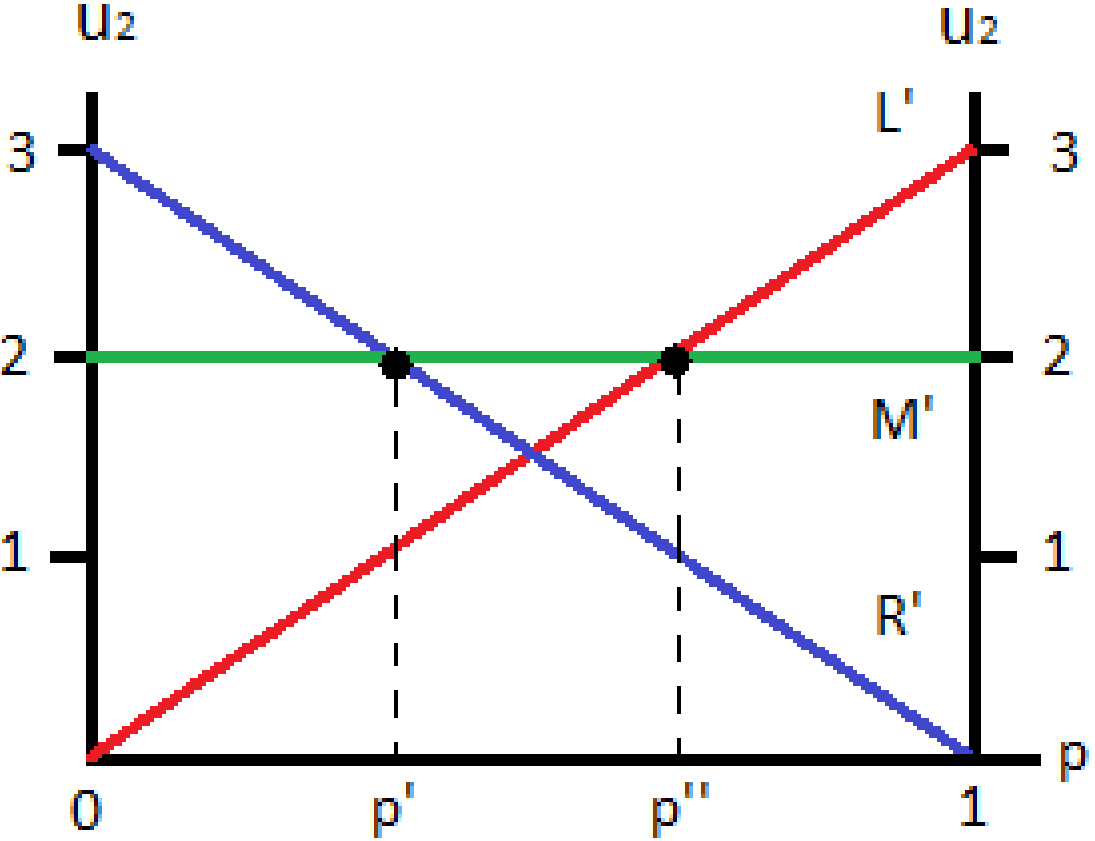
\includegraphics[width=1.1\columnwidth]{figures/Gibbons_4_1_b_E[u]}
      \vfill\null
    \end{multicols}
\end{frame}
\begin{frame}{PS10, Ex. 5.b: Extensive form games (Perfect Bayesian Equilibria)}
    Exercise 4.1.b in Gibbons (p. 245). In the following extensive-form games, derive the normal-form game and find all the pure-strategy NE, SPNE, and PBE.
    \vspace{-8pt}
    \begin{multicols}{2}
      \begin{table}
        \begin{tabular}{l|c|c|c|}
          \multicolumn{1}{c}{} & \multicolumn{1}{c}{L'} & \multicolumn{1}{c}{M'} & \multicolumn{1}{c}{R'} \\\cline{2-4}
          L [p]   & 1, \color{blue}3 & 1, 2 & \textcolor{red}{4}, 0 \\\cline{2-4}
          M [1-p] & \textcolor{red}{4}, 0 & 0, 2 & 3, \color{blue}3 \\\cline{2-4}
          R       & 2, \color{blue}4 & \textcolor{red}{2}, \color{blue}4 & 2, \color{blue}4 \\\cline{2-4}
        \end{tabular}
      \end{table} \vspace{-4pt}
      \begin{itemize}
        \item[PSNE:] $\{(R,M')\}$
        \item[SPNE =] PSNE, due to no proper subgames.
        \item[PBE:]
      \end{itemize} \vspace{-4pt}
      Given her beliefs, find P2's expected utility of $L'$, $M'$, and $R'$ respectively: \vspace{-4pt}
      \begin{align*}
        \mathbb{E}[u_2(L')|p]&=3p+0[1-p]=3p\\
        \mathbb{E}[u_2(M')|p]&=2p+2[1-p]=2\\
        \mathbb{E}[u_2(R')|p]&=0p+3[1-p]=3-3p
      \end{align*}
      P2 is indifferent at $p'$ and $p''$: \vspace{-4pt}
      \begin{align*}
        \mathbb{E}[u_2(M')]\text{=}\mathbb{E}[u_2(R')]&\Rightarrow 2\text{=3-3}p\Rightarrow p'\text{=}1/3\\
        \mathbb{E}[u_2(L')]\text{=}\mathbb{E}[u_2(M')]&\Rightarrow 3p\text{=}2\Rightarrow p''\text{=}2/3\\
      \end{align*}
      \vfill\null\columnbreak
      \begin{figure}[!h]
        \center \def\svgwidth{1.1\columnwidth}
        \import{figures/}{Gibbons_4_1_b.pdf_tex}
      \end{figure}
      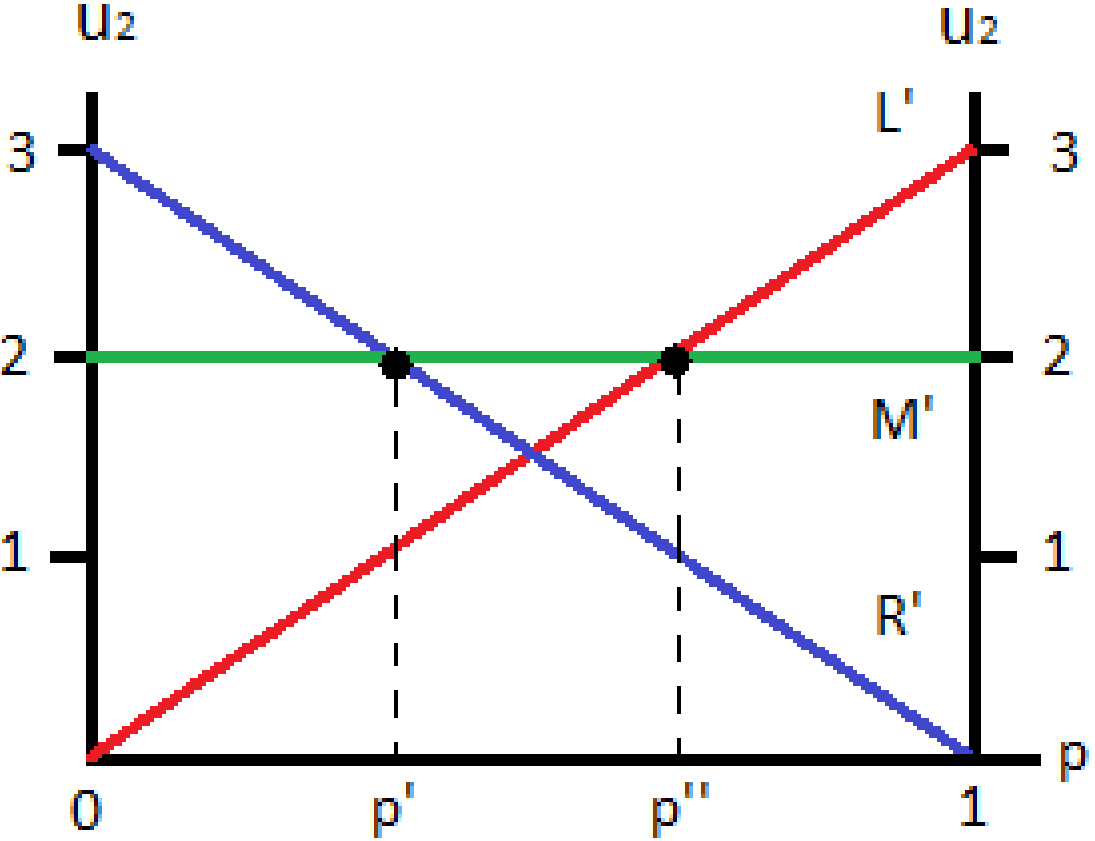
\includegraphics[width=1.1\columnwidth]{figures/Gibbons_4_1_b_E[u]}
      \vfill\null
    \end{multicols}
\end{frame}
\begin{frame}{PS10, Ex. 5.b: Extensive form games (Perfect Bayesian Equilibria)}
    Exercise 4.1.b in Gibbons (p. 245). In the following extensive-form games, derive the normal-form game and find all the pure-strategy NE, SPNE, and PBE.
    \vspace{-10pt}
    \begin{multicols}{2}
      \begin{table}
        \begin{tabular}{l|c|c|c|}
          \multicolumn{1}{c}{} & \multicolumn{1}{c}{L'} & \multicolumn{1}{c}{M'} & \multicolumn{1}{c}{R'} \\\cline{2-4}
          L [p]   & 1, \color{blue}3 & 1, 2 & \textcolor{red}{4}, 0 \\\cline{2-4}
          M [1-p] & \textcolor{red}{4}, 0 & 0, 2 & 3, \color{blue}3 \\\cline{2-4}
          R       & 2, \color{blue}4 & \textcolor{red}{2}, \color{blue}4 & 2, \color{blue}4 \\\cline{2-4}
        \end{tabular}
      \end{table} \vspace{-8pt}
      \begin{itemize}
        \item[PSNE:] $\{(R,M')\}$
        \item[SPNE =] PSNE, due to no proper subgames.
        \item[PBE:]
      \end{itemize} \vspace{-6pt}
      Given her beliefs, find P2's expected utility of $L'$, $M'$, and $R'$ respectively: \vspace{-6pt}
      \begin{align*}
        \mathbb{E}[u_2(L')|p]&=3p+0[1-p]=3p\\
        \mathbb{E}[u_2(M')|p]&=2p+2[1-p]=2\\
        \mathbb{E}[u_2(R')|p]&=0p+3[1-p]=3-3p
      \end{align*}
      P2 is indifferent at $p'$ and $p''$: \vspace{-6pt}
      \begin{align*}
        \mathbb{E}[u_2(M')]\text{=}\mathbb{E}[u_2(R')]&\Rightarrow 2\text{=3-3}p\Rightarrow p'\text{=}1/3\\
        \mathbb{E}[u_2(L')]\text{=}\mathbb{E}[u_2(M')]&\Rightarrow 3p\text{=}2\Rightarrow p''\text{=}2/3
      \end{align*}
      \textbf{Writing up the $\bm{BR_1}$'s, are they consistent with the beliefs of P2 for the relevant interval $\bm{[0,p'],[p',p''],[p'',1]}$?}
      \vfill\null\columnbreak
      \begin{figure}[!h]
        \center \def\svgwidth{1.1\columnwidth}
        \import{figures/}{Gibbons_4_1_b.pdf_tex}
      \end{figure}
      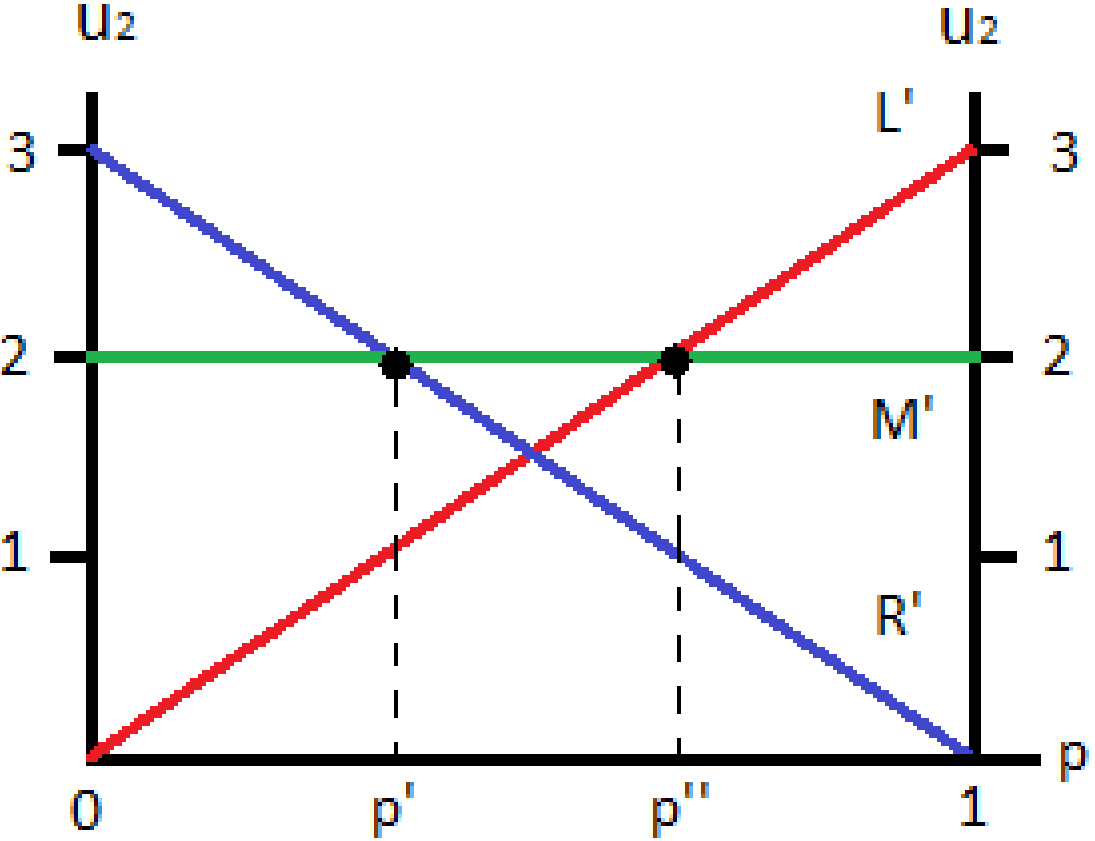
\includegraphics[width=1.1\columnwidth]{figures/Gibbons_4_1_b_E[u]}
      \vfill\null
    \end{multicols}
\end{frame}
\begin{frame}{PS10, Ex. 5.b: Extensive form games (Perfect Bayesian Equilibria)}
    Exercise 4.1.b in Gibbons (p. 245). In the following extensive-form games, derive the normal-form game and find all the pure-strategy NE, SPNE, and PBE.
    \vspace{-10pt}
    \begin{multicols}{2}
      \begin{table}
        \begin{tabular}{l|c|c|c|}
          \multicolumn{1}{c}{} & \multicolumn{1}{c}{L'} & \multicolumn{1}{c}{M'} & \multicolumn{1}{c}{R'} \\\cline{2-4}
          L [p]   & 1, \color{blue}3 & 1, 2 & \textcolor{red}{4}, 0 \\\cline{2-4}
          M [1-p] & \textcolor{red}{4}, 0 & 0, 2 & 3, \color{blue}3 \\\cline{2-4}
          R       & 2, \color{blue}4 & \textcolor{red}{2}, \color{blue}4 & 2, \color{blue}4 \\\cline{2-4}
        \end{tabular}
      \end{table} \vspace{-8pt}
      \begin{itemize}
        \item[PSNE:] $\{(R,M')\}$
        \item[SPNE =] PSNE, due to no proper subgames.
        \item[PBE:] \textbf{Now, write up the PBE.}
      \end{itemize} \vspace{-6pt}
      Given her beliefs, find P2's expected utility of $L'$, $M'$, and $R'$ respectively: \vspace{-6pt}
      \begin{align*}
        \mathbb{E}[u_2(L')|p]&=3p+0[1-p]=3p\\
        \mathbb{E}[u_2(M')|p]&=2p+2[1-p]=2\\
        \mathbb{E}[u_2(R')|p]&=0p+3[1-p]=3-3p
      \end{align*}
      P2 is indifferent at $p'$ and $p''$: \vspace{-6pt}
      \begin{align*}
        \mathbb{E}[u_2(M')]\text{=}\mathbb{E}[u_2(R')]&\Rightarrow 2\text{=3-3}p\Rightarrow p'\text{=}1/3\\
        \mathbb{E}[u_2(L')]\text{=}\mathbb{E}[u_2(M')]&\Rightarrow 3p\text{=}2\Rightarrow p''\text{=}2/3
      \end{align*} \vspace{-22pt}
      \begin{align*}
        p\leq1/3&\text{:}\ BR_1(R')=L\rightarrow\text{P2 deviates to }L'\\
        p\text{$\in$}{\textstyle\left[\frac{1}{3},\frac{2}{3}\right]}&\text{:}\ BR_1(M')=R\rightarrow\text{no deviation}\\
        p\geq2/3&\text{:}\ BR_1(L')=M\rightarrow\text{P2 deviates to }R'
      \end{align*}
      \vfill\null\columnbreak
      \begin{figure}[!h]
        \center \def\svgwidth{1.1\columnwidth}
        \import{figures/}{Gibbons_4_1_b.pdf_tex}
      \end{figure}
      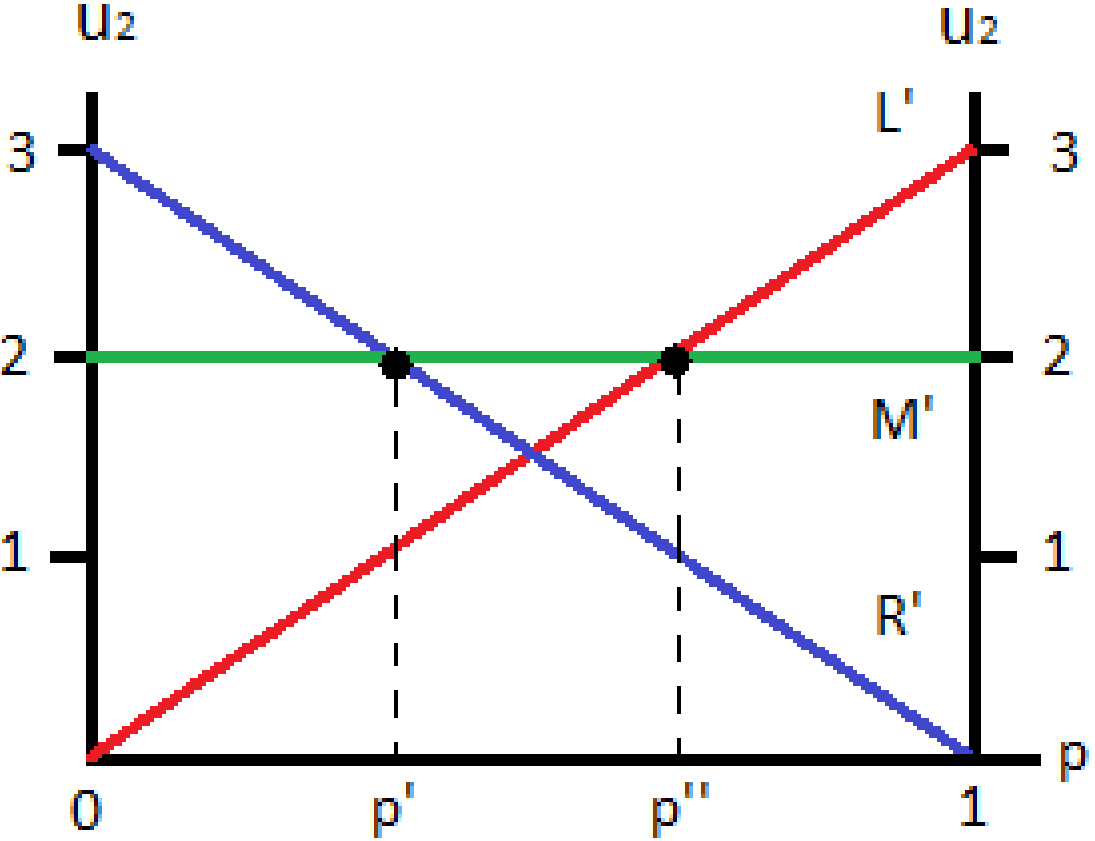
\includegraphics[width=1.1\columnwidth]{figures/Gibbons_4_1_b_E[u]}
      \vfill\null
    \end{multicols}
\end{frame}
\begin{frame}{PS10, Ex. 5.b: Extensive form games (Perfect Bayesian Equilibria)}
    Exercise 4.1.b in Gibbons (p. 245). In the following extensive-form games, derive the normal-form game and find all the pure-strategy NE, SPNE, and PBE.
    \vspace{-9pt}
    \begin{multicols}{2}
      \begin{table}
        \begin{tabular}{l|c|c|c|}
          \multicolumn{1}{c}{} & \multicolumn{1}{c}{L'} & \multicolumn{1}{c}{M'} & \multicolumn{1}{c}{R'} \\\cline{2-4}
          L [p]   & 1, \color{blue}3 & 1, 2 & \textcolor{red}{4}, 0 \\\cline{2-4}
          M [1-p] & \textcolor{red}{4}, 0 & 0, 2 & 3, \color{blue}3 \\\cline{2-4}
          R       & 2, \color{blue}4 & \textcolor{red}{2}, \color{blue}4 & 2, \color{blue}4 \\\cline{2-4}
        \end{tabular}
      \end{table} \vspace{-8pt}
      \begin{itemize}
        \item[PSNE:] $\{(R,M')\}$
        \item[SPNE =] PSNE, due to no proper subgames.
        \item[PBE:] $\bm{\left\{(R,M'),p\in\left[\frac{1}{3},\frac{2}{3}\right]\right\}}$
      \end{itemize} \vspace{-6pt}
      Given her beliefs, find P2's expected utility of $L'$, $M'$, and $R'$ respectively: \vspace{-6pt}
      \begin{align*}
        \mathbb{E}[u_2(L')|p]&=3p+0[1-p]=3p\\
        \mathbb{E}[u_2(M')|p]&=2p+2[1-p]=2\\
        \mathbb{E}[u_2(R')|p]&=0p+3[1-p]=3-3p
      \end{align*}
      P2 is indifferent at $p'$ and $p''$: \vspace{-6pt}
      \begin{align*}
        \mathbb{E}[u_2(M')]\text{=}\mathbb{E}[u_2(R')]&\Rightarrow 2\text{=3-3}p\Rightarrow p'\text{=}1/3\\
        \mathbb{E}[u_2(L')]\text{=}\mathbb{E}[u_2(M')]&\Rightarrow 3p\text{=}2\Rightarrow p''\text{=}2/3
      \end{align*} \vspace{-22pt}
      \begin{align*}
        p\leq1/3&\text{:}\ BR_1(R')=L\rightarrow\text{P2 deviates to }L'\\
        p\text{$\in$}{\textstyle\left[\frac{1}{3},\frac{2}{3}\right]}&\text{:}\ BR_1(M')=R\rightarrow\text{no deviation}\\
        p\geq2/3&\text{:}\ BR_1(L')=M\rightarrow\text{P2 deviates to }R'
      \end{align*}
      \vfill\null\columnbreak
      \begin{figure}[!h]
        \center \def\svgwidth{1.1\columnwidth}
        \import{figures/}{Gibbons_4_1_b.pdf_tex}
      \end{figure}
      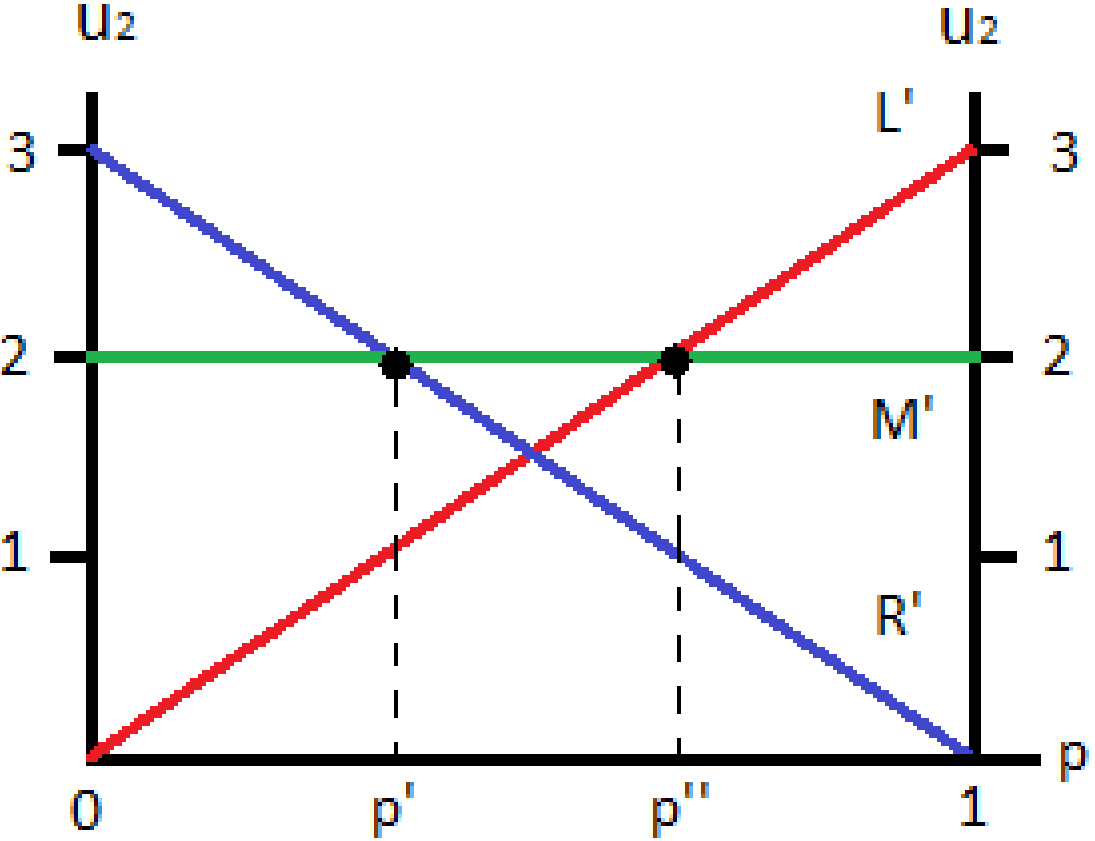
\includegraphics[width=1.1\columnwidth]{figures/Gibbons_4_1_b_E[u]}
      \vfill\null
    \end{multicols}
\end{frame}



\section{PS10, Ex. 6: Extensive form game (mixed-strategy Perfect Bayesian Equilibrium)}

\begin{frame}{PS10, Ex. 6: Extensive form game (mixed-strategy PBE)}
    Exercise 4.2 in Gibbons (p. 245). (i) Show that there does not exist a pure-strategy PBE in the following extensive-form game. (ii) What is the mixed-strategy PBE?
    \begin{multicols}{2}
      \vfill\null\columnbreak
      \begin{figure}[!h]
        \center \def\svgwidth{1.1\columnwidth}
        \import{figures/}{Gibbons_4_2_i.pdf_tex}
      \end{figure}
      \vfill\null
    \end{multicols}
\end{frame}

\begin{frame}{PS10, Ex. 6 (i): Extensive form game (mixed-strategy PBE)}
    (i) Show that there does not exist a pure-strategy perfect Bayesian equilibrium.
    \begin{multicols}{2}
      \begin{table}
        \begin{tabular}{l|c|c|}
          \multicolumn{1}{c}{} & \multicolumn{1}{c}{L'} & \multicolumn{1}{c}{R'} \\\cline{2-3}
          L [p]   & 3, 0 & 0, 1 \\\cline{2-3}
          M [1-p] & 0, 1 & 3, 0 \\\cline{2-3}
          R       & 2, 2 & 2, 2 \\\cline{2-3}
        \end{tabular}
      \end{table} \vspace{-4pt}
      \vfill\null\columnbreak
      \begin{figure}[!h]
        \center \def\svgwidth{1.1\columnwidth}
        \import{figures/}{Gibbons_4_2_i.pdf_tex}
      \end{figure}
      \vfill\null
    \end{multicols}
\end{frame}
\begin{frame}{PS10, Ex. 6 (i): Extensive form game (mixed-strategy PBE)}
    (i) Show that there does not exist a pure-strategy perfect Bayesian equilibrium.
    \begin{multicols}{2}
      \begin{table}
        \begin{tabular}{l|c|c|}
          \multicolumn{1}{c}{} & \multicolumn{1}{c}{L'} & \multicolumn{1}{c}{R'} \\\cline{2-3}
          L [p]   & \textcolor{red}{3}, 0 & 0, \color{blue}1 \\\cline{2-3}
          M [1-p] & 0, \color{blue}1 & \textcolor{red}{3}, 0 \\\cline{2-3}
          R       & 2, \color{blue}2 & 2, \color{blue}2 \\\cline{2-3}
        \end{tabular}
      \end{table} \vspace{-4pt}
      \vfill\null\columnbreak
      \begin{figure}[!h]
        \center \def\svgwidth{1.1\columnwidth}
        \import{figures/}{Gibbons_4_2_i.pdf_tex}
      \end{figure}
      \vfill\null
    \end{multicols}
\end{frame}
\begin{frame}{PS10, Ex. 6 (i): Extensive form game (mixed-strategy PBE)}
    (i) Show that there does not exist a pure-strategy perfect Bayesian equilibrium.
    \begin{multicols}{2}
      \begin{table}
        \begin{tabular}{l|c|c|}
          \multicolumn{1}{c}{} & \multicolumn{1}{c}{L'} & \multicolumn{1}{c}{R'} \\\cline{2-3}
          L [p]   & \textcolor{red}{3}, 0 & 0, \color{blue}1 \\\cline{2-3}
          M [1-p] & 0, \color{blue}1 & \textcolor{red}{3}, 0 \\\cline{2-3}
          R       & 2, \color{blue}2 & 2, \color{blue}2 \\\cline{2-3}
        \end{tabular}
      \end{table} \vspace{-4pt}
      From the bi-matrix it is clear there is no equilibrium in pure strategies as one of the players would always want to deviate.
      \vfill\null\columnbreak
      \begin{figure}[!h]
        \center \def\svgwidth{1.1\columnwidth}
        \import{figures/}{Gibbons_4_2_i.pdf_tex}
      \end{figure}
      \vfill\null
    \end{multicols}
\end{frame}

\begin{frame}{PS10, Ex. 6 (ii): Extensive form game (mixed-strategy PBE)}
    (ii) What is the mixed-strategy PBE? \vspace{-8pt}
    \begin{multicols}{2}
      \begin{table}
        \begin{tabular}{l|c|c|}
          \multicolumn{1}{c}{} & \multicolumn{1}{c}{L'} & \multicolumn{1}{c}{R'} \\\cline{2-3}
          L [p]   & \textcolor{red}{3}, 0 & 0, \color{blue}1 \\\cline{2-3}
          M [1-p] & 0, \color{blue}1 & \textcolor{red}{3}, 0 \\\cline{2-3}
          R       & 2, \color{blue}2 & 2, \color{blue}2 \\\cline{2-3}
        \end{tabular}
      \end{table} \vspace{-4pt}
      \vfill\null\columnbreak
      \begin{figure}[!h]
        \center \def\svgwidth{1.1\columnwidth}
        \import{figures/}{Gibbons_4_2_i.pdf_tex}
      \end{figure}
      \vfill\null
    \end{multicols}
\end{frame}
\begin{frame}{PS10, Ex. 6 (ii): Extensive form game (mixed-strategy PBE)}
    (ii) What is the mixed-strategy PBE? \vspace{-8pt}
    \begin{multicols}{2}
      \begin{table}
        \begin{tabular}{l|c|c|}
          \multicolumn{1}{c}{} & \multicolumn{1}{c}{L' [q]} & \multicolumn{1}{c}{R' [1-q]} \\\cline{2-3}
          L [p]   & \textcolor{red}{3}, 0 & 0, \color{blue}1 \\\cline{2-3}
          M [1-p] & 0, \color{blue}1 & \textcolor{red}{3}, 0 \\\cline{2-3}
          R       & 2, \color{blue}2 & 2, \color{blue}2 \\\cline{2-3}
        \end{tabular}
      \end{table} \vspace{-4pt}
      Assume that P2 plays $L'$ and $R'$ with probability $q$ and $1-q$ respectively.\\\smallskip
      \textbf{Given his beliefs, find P1's expected utility of $\bm{L}$, $\bm{M}$, and $\bm{R}$ respectively.}
      \vfill\null\columnbreak
      \begin{figure}[!h]
        \center \def\svgwidth{1.1\columnwidth}
        \import{figures/}{Gibbons_4_2_ii.pdf_tex}
      \end{figure}
      \vfill\null
    \end{multicols}
\end{frame}
\begin{frame}{PS10, Ex. 6 (ii): Extensive form game (mixed-strategy PBE)}
    (ii) What is the mixed-strategy PBE? \vspace{-8pt}
    \begin{multicols}{2}
      \begin{table}
        \begin{tabular}{l|c|c|}
          \multicolumn{1}{c}{} & \multicolumn{1}{c}{L' [q]} & \multicolumn{1}{c}{R' [1-q]} \\\cline{2-3}
          L [p]   & \textcolor{red}{3}, 0 & 0, \color{blue}1 \\\cline{2-3}
          M [1-p] & 0, \color{blue}1 & \textcolor{red}{3}, 0 \\\cline{2-3}
          R       & 2, \color{blue}2 & 2, \color{blue}2 \\\cline{2-3}
        \end{tabular}
      \end{table} \vspace{-4pt}
      Assume that P2 plays $L'$ and $R'$ with probability $q$ and $1-q$ respectively.\\\smallskip
      Given his beliefs, find P1's expected utility of $L$, $M$, and $R$ respectively: \vspace{-4pt}
      \begin{align*}
        \mathbb{E}[u_1(L)|q]&=3q+0[1-q]=3q\\
        \mathbb{E}[u_1(M)|q]&=0q+3[1-q]=3-3q\\
        \mathbb{E}[u_1(R)]&=2
      \end{align*}
      \vfill\null\columnbreak
      \begin{figure}[!h]
        \center \def\svgwidth{1.1\columnwidth}
        \import{figures/}{Gibbons_4_2_ii.pdf_tex}
      \end{figure}
      \vfill\null
    \end{multicols}
\end{frame}
\begin{frame}{PS10, Ex. 6 (ii): Extensive form game (mixed-strategy PBE)}
    (ii) What is the mixed-strategy PBE? \vspace{-8pt}
    \begin{multicols}{2}
      \begin{table}
        \begin{tabular}{l|c|c|}
          \multicolumn{1}{c}{} & \multicolumn{1}{c}{L' [q]} & \multicolumn{1}{c}{R' [1-q]} \\\cline{2-3}
          L [p]   & \textcolor{red}{3}, 0 & 0, \color{blue}1 \\\cline{2-3}
          M [1-p] & 0, \color{blue}1 & \textcolor{red}{3}, 0 \\\cline{2-3}
          R       & 2, \color{blue}2 & 2, \color{blue}2 \\\cline{2-3}
        \end{tabular}
      \end{table} \vspace{-4pt}
      Assume that P2 plays $L'$ and $R'$ with probability $q$ and $1-q$ respectively.\\\smallskip
      Given his beliefs, find P1's expected utility of $L$, $M$, and $R$ respectively: \vspace{-4pt}
      \begin{align*}
        \mathbb{E}[u_1(L)|q]&=3q+0[1-q]=3q\\
        \mathbb{E}[u_1(M)|q]&=0q+3[1-q]=3-3q\\
        \mathbb{E}[u_1(R)]&=2
      \end{align*}
      \textbf{Draw the expected utility of each choice as functions of \textit{q}.}
      \vfill\null\columnbreak
      \begin{figure}[!h]
        \center \def\svgwidth{1.1\columnwidth}
        \import{figures/}{Gibbons_4_2_ii.pdf_tex}
      \end{figure}
      \vfill\null
    \end{multicols}
\end{frame}
\begin{frame}{PS10, Ex. 6 (ii): Extensive form game (mixed-strategy PBE)}
    (ii) What is the mixed-strategy PBE? \vspace{-8pt}
    \begin{multicols}{2}
      \begin{table}
        \begin{tabular}{l|c|c|}
          \multicolumn{1}{c}{} & \multicolumn{1}{c}{L' [q]} & \multicolumn{1}{c}{R' [1-q]} \\\cline{2-3}
          L [p]   & \textcolor{red}{3}, 0 & 0, \color{blue}1 \\\cline{2-3}
          M [1-p] & 0, \color{blue}1 & \textcolor{red}{3}, 0 \\\cline{2-3}
          R       & 2, \color{blue}2 & 2, \color{blue}2 \\\cline{2-3}
        \end{tabular}
      \end{table} \vspace{-4pt}
      Assume that P2 plays $L'$ and $R'$ with probability $q$ and $1-q$ respectively.\\\smallskip
      Given his beliefs, find P1's expected utility of $L$, $M$, and $R$ respectively: \vspace{-4pt}
      \begin{align*}
        \mathbb{E}[u_1(L)|q]&=3q+0[1-q]=3q\\
        \mathbb{E}[u_1(M)|q]&=0q+3[1-q]=3-3q\\
        \mathbb{E}[u_1(R)]&=2
      \end{align*}
      \vfill\null\columnbreak
      \begin{figure}[!h]
        \center \def\svgwidth{1.1\columnwidth}
        \import{figures/}{Gibbons_4_2_ii.pdf_tex}
      \end{figure}
      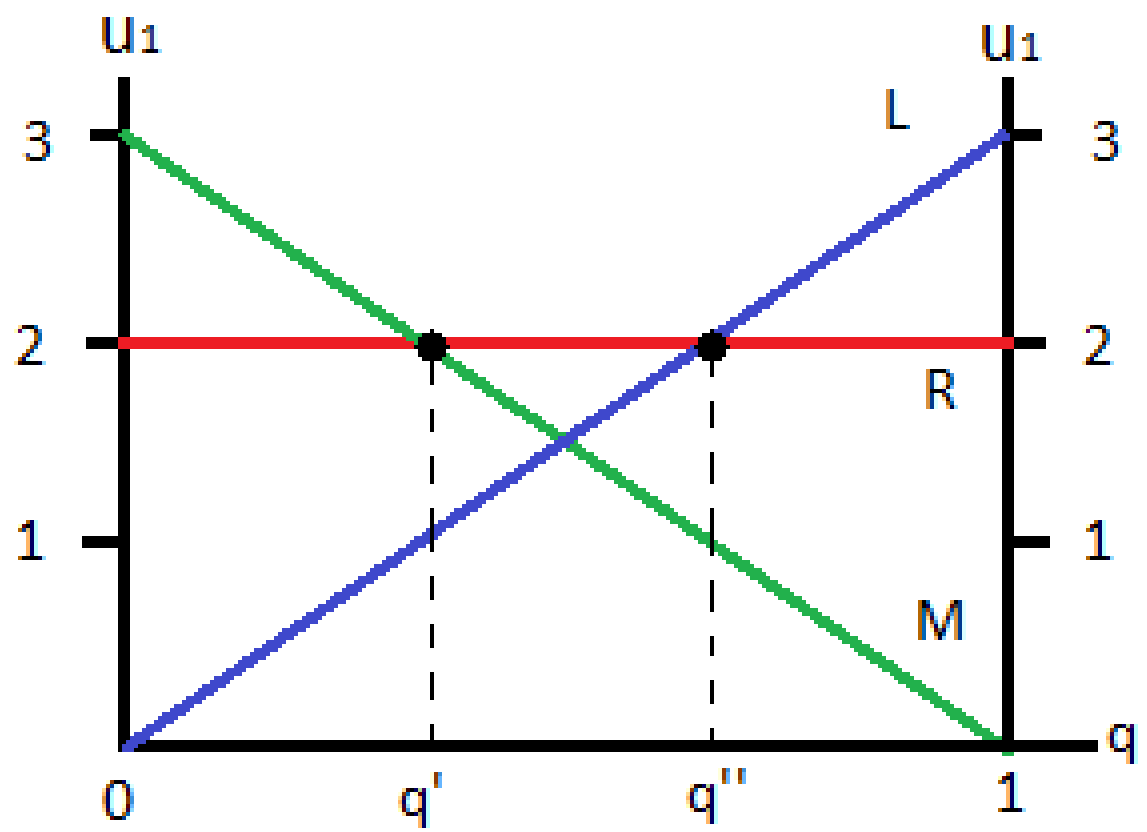
\includegraphics[width=1.1\columnwidth]{figures/Gibbons_4_2_E[u]}
      \vfill\null
    \end{multicols}
\end{frame}
\begin{frame}{PS10, Ex. 6 (ii): Extensive form game (mixed-strategy PBE)}
    (ii) What is the mixed-strategy PBE? \vspace{-8pt}
    \begin{multicols}{2}
      \begin{table}
        \begin{tabular}{l|c|c|}
          \multicolumn{1}{c}{} & \multicolumn{1}{c}{L' [q]} & \multicolumn{1}{c}{R' [1-q]} \\\cline{2-3}
          L [p]   & \textcolor{red}{3}, 0 & 0, \color{blue}1 \\\cline{2-3}
          M [1-p] & 0, \color{blue}1 & \textcolor{red}{3}, 0 \\\cline{2-3}
          R       & 2, \color{blue}2 & 2, \color{blue}2 \\\cline{2-3}
        \end{tabular}
      \end{table} \vspace{-4pt}
      Assume that P2 plays $L'$ and $R'$ with probability $q$ and $1-q$ respectively.\\\smallskip
      Given his beliefs, find P1's expected utility of $L$, $M$, and $R$ respectively: \vspace{-4pt}
      \begin{align*}
        \mathbb{E}[u_1(L)|q]&=3q+0[1-q]=3q\\
        \mathbb{E}[u_1(M)|q]&=0q+3[1-q]=3-3q\\
        \mathbb{E}[u_1(R)]&=2
      \end{align*}
      \textbf{Using the diagram and the expected utility functions, find the intersections $q'$ and $q''$.}
      \vfill\null\columnbreak
      \begin{figure}[!h]
        \center \def\svgwidth{1.1\columnwidth}
        \import{figures/}{Gibbons_4_2_ii.pdf_tex}
      \end{figure}
      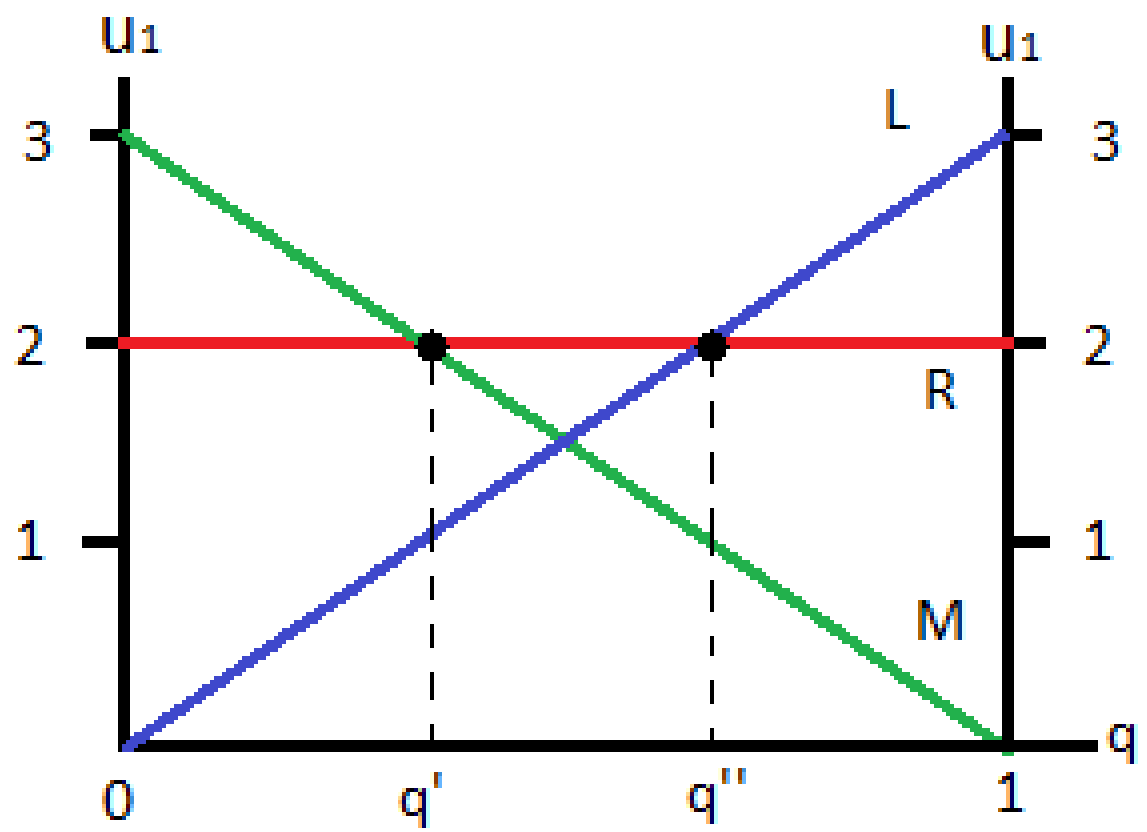
\includegraphics[width=1.1\columnwidth]{figures/Gibbons_4_2_E[u]}
      \vfill\null
    \end{multicols}
\end{frame}
\begin{frame}{PS10, Ex. 6 (ii): Extensive form game (mixed-strategy PBE)}
    (ii) What is the mixed-strategy PBE? \vspace{-8pt}
    \begin{multicols}{2}
      \begin{table}
        \begin{tabular}{l|c|c|}
          \multicolumn{1}{c}{} & \multicolumn{1}{c}{L' [q]} & \multicolumn{1}{c}{R' [1-q]} \\\cline{2-3}
          L [p]   & \textcolor{red}{3}, 0 & 0, \color{blue}1 \\\cline{2-3}
          M [1-p] & 0, \color{blue}1 & \textcolor{red}{3}, 0 \\\cline{2-3}
          R       & 2, \color{blue}2 & 2, \color{blue}2 \\\cline{2-3}
        \end{tabular}
      \end{table} \vspace{-4pt}
      Assume that P2 plays $L'$ and $R'$ with probability $q$ and $1-q$ respectively.\\\smallskip
      Given his beliefs, find P1's expected utility of $L$, $M$, and $R$ respectively: \vspace{-4pt}
      \begin{align*}
        \mathbb{E}[u_1(L)|q]&=3q+0[1-q]=3q\\
        \mathbb{E}[u_1(M)|q]&=0q+3[1-q]=3-3q\\
        \mathbb{E}[u_1(R)]&=2
      \end{align*}
      P1 is indifferent at $q'$ and $q''$: \vspace{-6pt}
      \begin{align*}
        \mathbb{E}[u_1(M)]\text{=}\mathbb{E}[u_1(R)]&\Rightarrow \text{3-3}q\text{=}2\Rightarrow q'\text{=}1/3\\
        \mathbb{E}[u_1(L)]\text{=}\mathbb{E}[u_1(R)]&\Rightarrow 3q\text{=}2\Rightarrow q''\text{=}2/3
      \end{align*}
      \vfill\null\columnbreak
      \begin{figure}[!h]
        \center \def\svgwidth{1.1\columnwidth}
        \import{figures/}{Gibbons_4_2_ii.pdf_tex}
      \end{figure}
      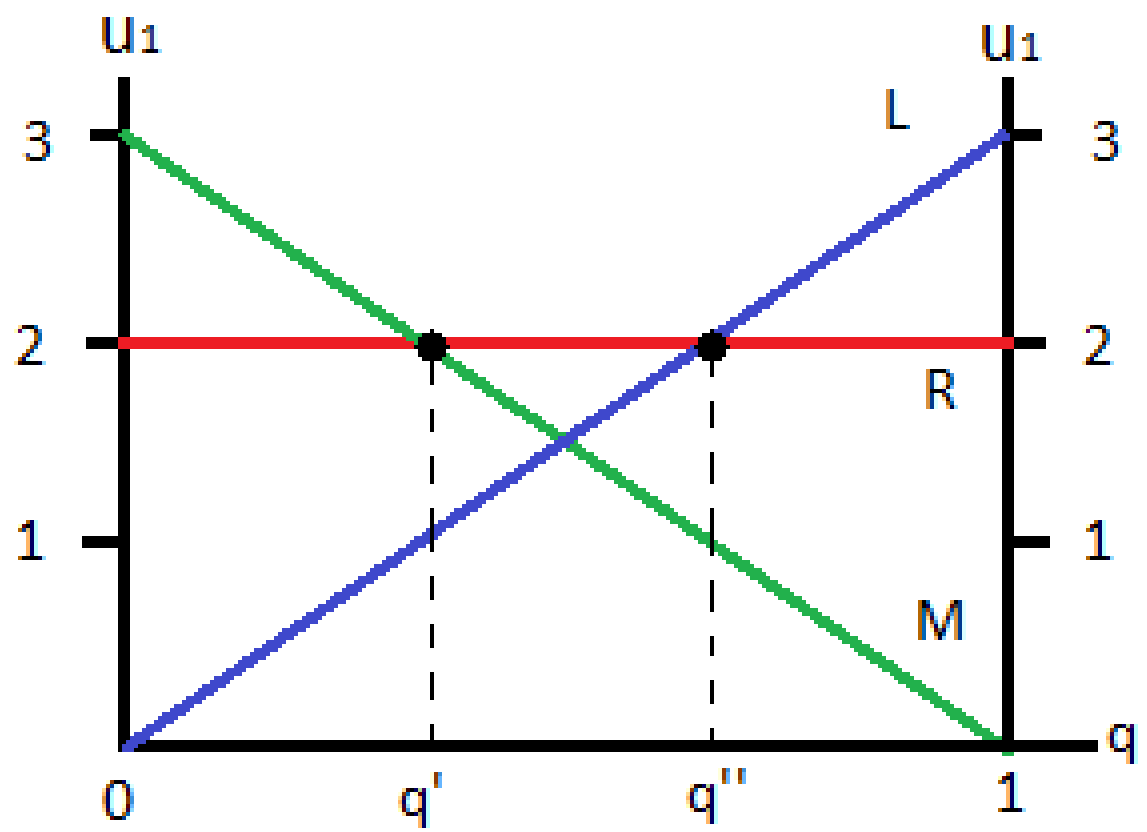
\includegraphics[width=1.1\columnwidth]{figures/Gibbons_4_2_E[u]}
      \vfill\null
    \end{multicols}
\end{frame}
\begin{frame}{PS10, Ex. 6 (ii): Extensive form game (mixed-strategy PBE)}
    (ii) What is the mixed-strategy PBE? \vspace{-8pt}
    \begin{multicols}{2}
      \begin{table}
        \begin{tabular}{l|c|c|}
          \multicolumn{1}{c}{} & \multicolumn{1}{c}{L' [q]} & \multicolumn{1}{c}{R' [1-q]} \\\cline{2-3}
          L [p]   & \textcolor{red}{3}, 0 & 0, \color{blue}1 \\\cline{2-3}
          M [1-p] & 0, \color{blue}1 & \textcolor{red}{3}, 0 \\\cline{2-3}
          R       & 2, \color{blue}2 & 2, \color{blue}2 \\\cline{2-3}
        \end{tabular}
      \end{table} \vspace{-4pt}
      Assume that P2 plays $L'$ and $R'$ with probability $q$ and $1-q$ respectively.\\\smallskip
      Given his beliefs, find P1's expected utility of $L$, $M$, and $R$ respectively: \vspace{-4pt}
      \begin{align*}
        \mathbb{E}[u_1(L)|q]&=3q+0[1-q]=3q\\
        \mathbb{E}[u_1(M)|q]&=0q+3[1-q]=3-3q\\
        \mathbb{E}[u_1(R)]&=2
      \end{align*}
      P1 is indifferent at $q'$ and $q''$: \vspace{-6pt}
      \begin{align*}
        \mathbb{E}[u_1(M)]\text{=}\mathbb{E}[u_1(R)]&\Rightarrow \text{3-3}q\text{=}2\Rightarrow q'\text{=}1/3\\
        \mathbb{E}[u_1(L)]\text{=}\mathbb{E}[u_1(R)]&\Rightarrow 3q\text{=}2\Rightarrow q''\text{=}2/3
      \end{align*}
      \textbf{Writing up the $\bm{BR_2}$'s, are they consistent with the beliefs of P1 for the relevant interval $\bm{[0,q'],[q',q''],[q'',1]}$?}
      \vfill\null\columnbreak
      \begin{figure}[!h]
        \center \def\svgwidth{1.1\columnwidth}
        \import{figures/}{Gibbons_4_2_ii.pdf_tex}
      \end{figure}
      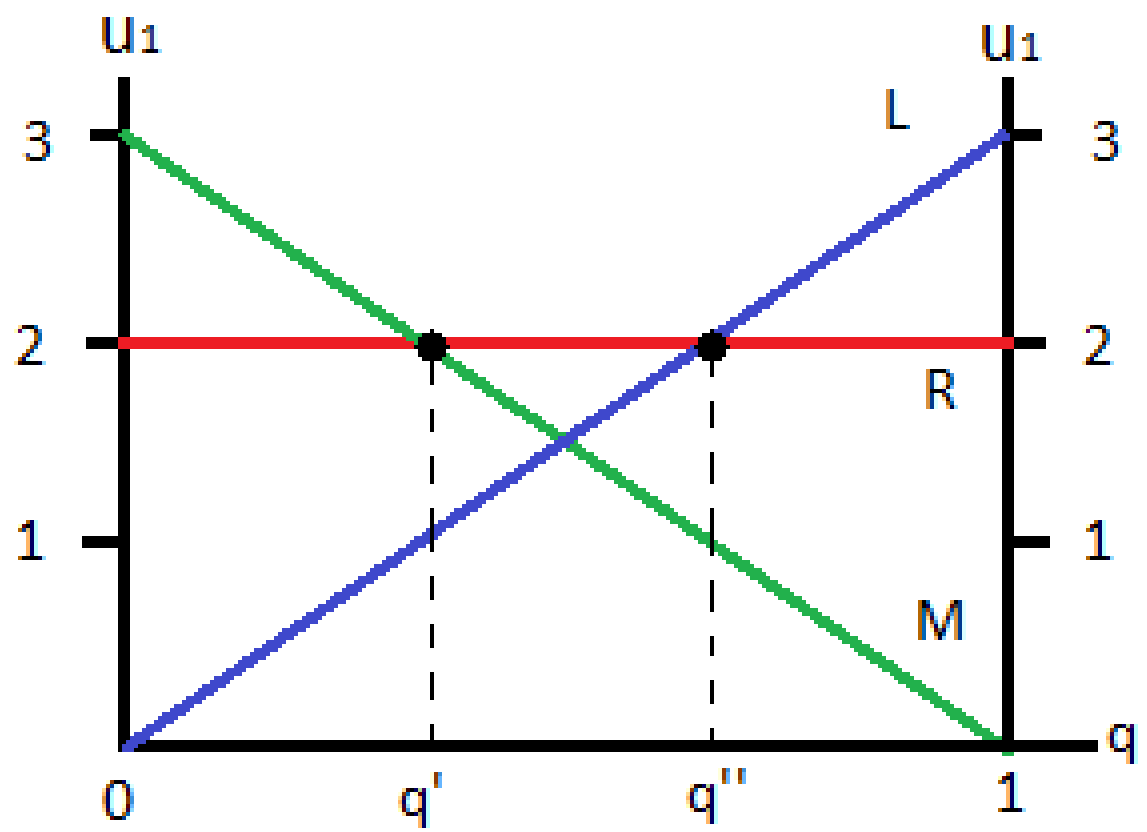
\includegraphics[width=1.1\columnwidth]{figures/Gibbons_4_2_E[u]}
      \vfill\null
    \end{multicols}
\end{frame}
\begin{frame}{PS10, Ex. 6 (ii): Extensive form game (mixed-strategy PBE)}
    (ii) What is the mixed-strategy PBE? \vspace{-8pt}
    \begin{multicols}{2}
      \begin{table}
        \begin{tabular}{l|c|c|}
          \multicolumn{1}{c}{} & \multicolumn{1}{c}{L' [q]} & \multicolumn{1}{c}{R' [1-q]} \\\cline{2-3}
          L [p]   & \textcolor{red}{3}, 0 & 0, \color{blue}1 \\\cline{2-3}
          M [1-p] & 0, \color{blue}1 & \textcolor{red}{3}, 0 \\\cline{2-3}
          R       & 2, \color{blue}2 & 2, \color{blue}2 \\\cline{2-3}
        \end{tabular}
      \end{table} \vspace{-4pt}
      Given his beliefs, find P1's expected utility of $L$, $M$, and $R$ respectively: \vspace{-4pt}
      \begin{align*}
        \mathbb{E}[u_1(L)|q]&=3q+0[1-q]=3q\\
        \mathbb{E}[u_1(M)|q]&=0q+3[1-q]=3-3q\\
        \mathbb{E}[u_1(R)]&=2
      \end{align*}
      P1 is indifferent at $q'$ and $q''$: \vspace{-6pt}
      \begin{align*}
        \mathbb{E}[u_1(M)]\text{=}\mathbb{E}[u_1(R)]&\Rightarrow \text{3-3}q\text{=}2\Rightarrow q'\text{=}1/3\\
        \mathbb{E}[u_1(L)]\text{=}\mathbb{E}[u_1(R)]&\Rightarrow 3q\text{=}2\Rightarrow q''\text{=}2/3
      \end{align*} \vspace{-16pt}
      \begin{align*}
        q\leq1/3&\text{:}\ BR_2(M)\text{=}L'\rightarrow\text{P1 deviates to }L\\
        q\text{$\in$}{\textstyle\left[\frac{1}{3},\frac{2}{3}\right]}&\text{:}\ \text{P1 plays }R\rightarrow\text{does P2 mix?}\\
        q\geq2/3&\text{:}\ BR_2(L)\text{=}R'\rightarrow\text{P2 deviates to }M
      \end{align*}
      \textbf{Find the beliefs $p$ such that P2 is indifferent between $L'$ and $R'$.}
      \vfill\null\columnbreak
      \begin{figure}[!h]
        \center \def\svgwidth{1.1\columnwidth}
        \import{figures/}{Gibbons_4_2_ii.pdf_tex}
      \end{figure}
      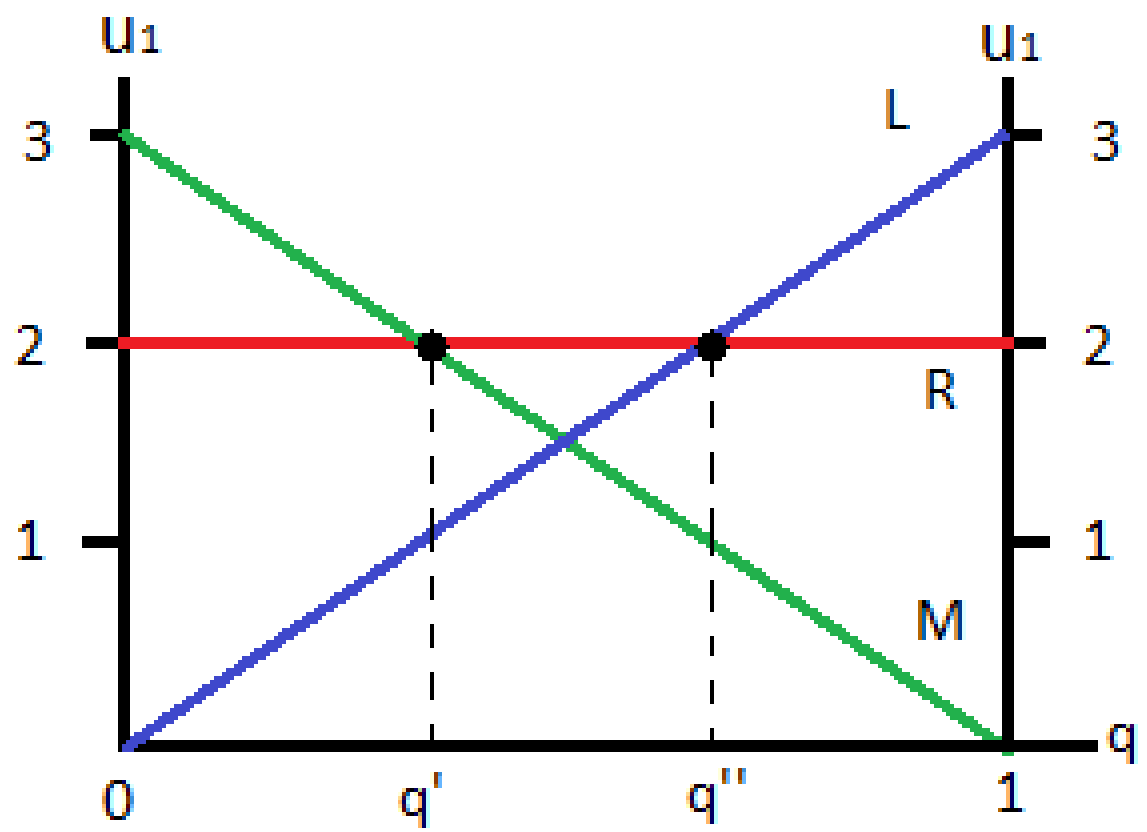
\includegraphics[width=1.1\columnwidth]{figures/Gibbons_4_2_E[u]}
      \vfill\null
    \end{multicols}
\end{frame}
\begin{frame}{PS10, Ex. 6 (ii): Extensive form game (mixed-strategy PBE)}
    (ii) What is the mixed-strategy PBE? \vspace{-8pt}
    \begin{multicols}{2}
      \begin{table}
        \begin{tabular}{l|c|c|}
          \multicolumn{1}{c}{} & \multicolumn{1}{c}{L' [q]} & \multicolumn{1}{c}{R' [1-q]} \\\cline{2-3}
          L [p]   & \textcolor{red}{3}, 0 & 0, \color{blue}1 \\\cline{2-3}
          M [1-p] & 0, \color{blue}1 & \textcolor{red}{3}, 0 \\\cline{2-3}
          R       & 2, \color{blue}2 & 2, \color{blue}2 \\\cline{2-3}
        \end{tabular}
      \end{table} \vspace{-4pt}
      Given his beliefs, find P1's expected utility of $L$, $M$, and $R$ respectively: \vspace{-4pt}
      \begin{align*}
        \mathbb{E}[u_1(L)|q]&=3q+0[1-q]=3q\\
        \mathbb{E}[u_1(M)|q]&=0q+3[1-q]=3-3q\\
        \mathbb{E}[u_1(R)]&=2
      \end{align*}
      P1 is indifferent at $q'$ and $q''$: \vspace{-6pt}
      \begin{align*}
        \mathbb{E}[u_1(M)]\text{=}\mathbb{E}[u_1(R)]&\Rightarrow \text{3-3}q\text{=}2\Rightarrow q'\text{=}1/3\\
        \mathbb{E}[u_1(L)]\text{=}\mathbb{E}[u_1(R)]&\Rightarrow 3q\text{=}2\Rightarrow q''\text{=}2/3
      \end{align*} \vspace{-16pt}
      \begin{align*}
        q\leq1/3&\text{:}\ BR_2(M)\text{=}L'\rightarrow\text{P1 deviates to }L\\
        q\text{$\in$}{\textstyle\left[\frac{1}{3},\frac{2}{3}\right]}&\text{:}\ \text{P1 plays }R\rightarrow\text{does P2 mix?}\\
        q\geq2/3&\text{:}\ BR_2(L)\text{=}R'\rightarrow\text{P2 deviates to }M
      \end{align*}
      P2 is indifferent if she believes that: \vspace{-6pt}
      \begin{align*}
        \mathbb{E}[u_2(L')]\text{=}\mathbb{E}[u_1(R')]\Rightarrow \text{0}p\text{+1[1-}p\text{]=}\text{1}p\text{+0[1-}p\text{]}\Rightarrow \text{1-}p\text{=}p\Rightarrow p^*\text{=}1/2
      \end{align*}
      \vfill\null\columnbreak
      \begin{figure}[!h]
        \center \def\svgwidth{1.1\columnwidth}
        \import{figures/}{Gibbons_4_2_ii.pdf_tex}
      \end{figure}
      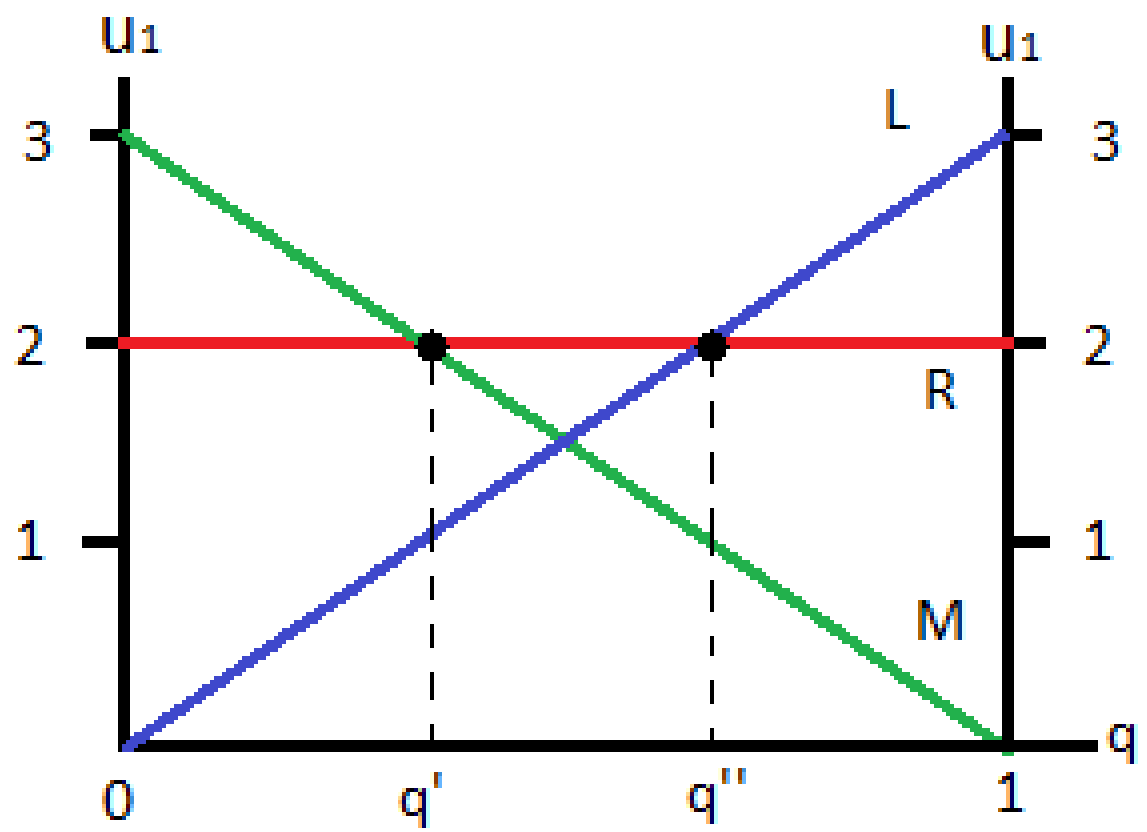
\includegraphics[width=1.1\columnwidth]{figures/Gibbons_4_2_E[u]}
      \vfill\null
    \end{multicols}
\end{frame}
\begin{frame}{PS10, Ex. 6 (ii): Extensive form game (mixed-strategy PBE)}
    (ii) What is the mixed-strategy PBE? \vspace{-8pt}
    \begin{multicols}{2}
      \begin{table}
        \begin{tabular}{l|c|c|}
          \multicolumn{1}{c}{} & \multicolumn{1}{c}{L' [q]} & \multicolumn{1}{c}{R' [1-q]} \\\cline{2-3}
          L [p]   & \textcolor{red}{3}, 0 & 0, \color{blue}1 \\\cline{2-3}
          M [1-p] & 0, \color{blue}1 & \textcolor{red}{3}, 0 \\\cline{2-3}
          R       & 2, \color{blue}2 & 2, \color{blue}2 \\\cline{2-3}
        \end{tabular}
      \end{table} \vspace{-4pt}
      Given his beliefs, find P1's expected utility of $L$, $M$, and $R$ respectively: \vspace{-4pt}
      \begin{align*}
        \mathbb{E}[u_1(L)|q]&=3q+0[1-q]=3q\\
        \mathbb{E}[u_1(M)|q]&=0q+3[1-q]=3-3q\\
        \mathbb{E}[u_1(R)]&=2
      \end{align*}
      P1 is indifferent at $q'$ and $q''$: \vspace{-6pt}
      \begin{align*}
        \mathbb{E}[u_1(M)]\text{=}\mathbb{E}[u_1(R)]&\Rightarrow \text{3-3}q\text{=}2\Rightarrow q'\text{=}1/3\\
        \mathbb{E}[u_1(L)]\text{=}\mathbb{E}[u_1(R)]&\Rightarrow 3q\text{=}2\Rightarrow q''\text{=}2/3
      \end{align*} \vspace{-16pt}
      \begin{align*}
        q\leq1/3&\text{:}\ BR_2(M)\text{=}L'\rightarrow\text{P1 deviates to }L\\
        q\text{$\in$}{\textstyle\left[\frac{1}{3},\frac{2}{3}\right]}&\text{:}\ \text{P1 plays }R\rightarrow\text{does P2 mix?}\\
        q\geq2/3&\text{:}\ BR_2(L)\text{=}R'\rightarrow\text{P2 deviates to }M
      \end{align*}
      P2 is indifferent if she believes that: \vspace{-6pt}
      \begin{align*}
        \mathbb{E}[u_2(L')]\text{=}\mathbb{E}[u_1(R')]&\Rightarrow \text{1-}p\text{=}p\Rightarrow p^*\text{=}1/2
      \end{align*}
      \textbf{Is $\bm{p=\frac{1}{2}}$ compatible with $\bm{q\in\left[\frac{1}{3},\frac{2}{3}\right]}$?}
      \vfill\null\columnbreak
      \begin{figure}[!h]
        \center \def\svgwidth{1.1\columnwidth}
        \import{figures/}{Gibbons_4_2_ii.pdf_tex}
      \end{figure}
      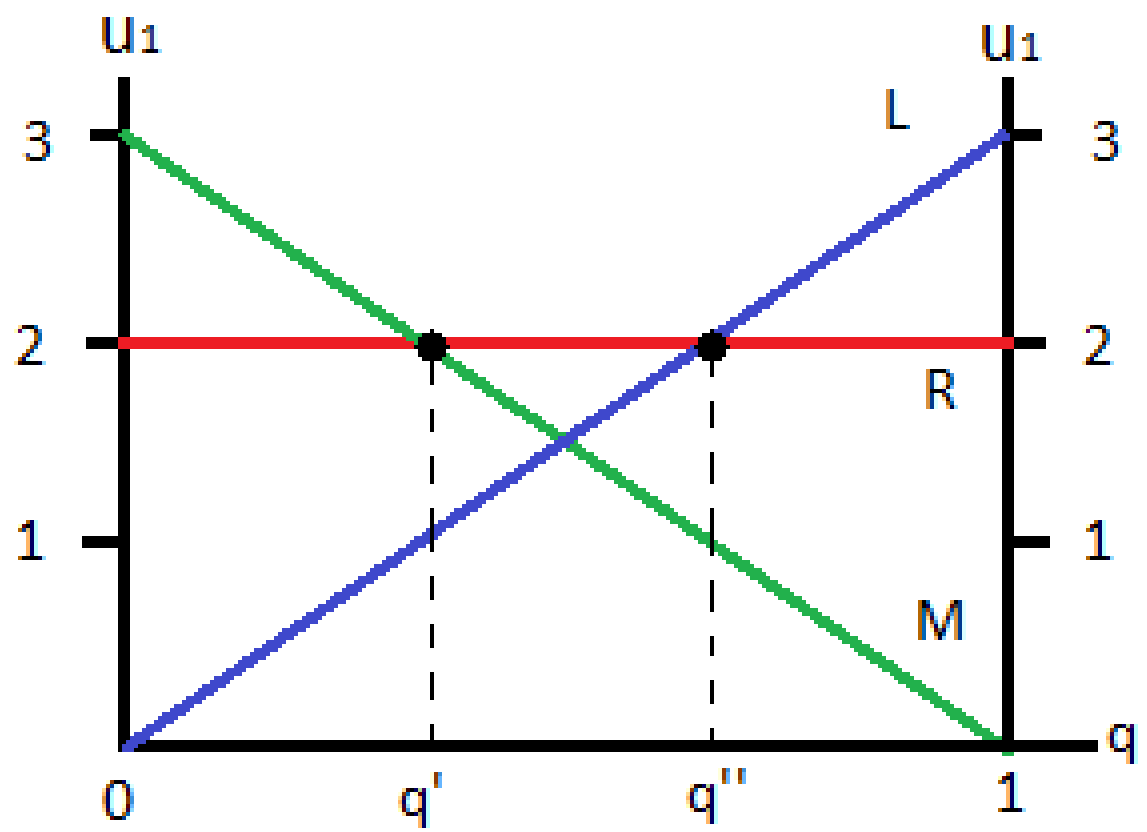
\includegraphics[width=1.1\columnwidth]{figures/Gibbons_4_2_E[u]}
      \vfill\null
    \end{multicols}
\end{frame}
\begin{frame}{PS10, Ex. 6 (ii): Extensive form game (mixed-strategy PBE)}
    (ii) What is the mixed-strategy PBE? \vspace{-10pt}
    \begin{multicols}{2}
      \begin{table}
        \begin{tabular}{l|c|c|}
          \multicolumn{1}{c}{} & \multicolumn{1}{c}{L' [q]} & \multicolumn{1}{c}{R' [1-q]} \\\cline{2-3}
          L [p]   & \textcolor{red}{3}, 0 & 0, \color{blue}1 \\\cline{2-3}
          M [1-p] & 0, \color{blue}1 & \textcolor{red}{3}, 0 \\\cline{2-3}
          R       & 2, \color{blue}2 & 2, \color{blue}2 \\\cline{2-3}
        \end{tabular}
      \end{table} \vspace{-6pt}
      P1's expected utility of $L$, $M$, and $R$: \vspace{-6pt}
      \begin{align*}
        \mathbb{E}[u_1(L)|q]&=3q+0[1-q]=3q\\
        \mathbb{E}[u_1(M)|q]&=0q+3[1-q]=3-3q\\
        \mathbb{E}[u_1(R)]&=2
      \end{align*}
      P1 is indifferent at $q'$ and $q''$: \vspace{-6pt}
      \begin{align*}
        \mathbb{E}[u_1(M)]\text{=}\mathbb{E}[u_1(R)]&\Rightarrow \text{3-3}q\text{=}2\Rightarrow q'\text{=}1/3\\
        \mathbb{E}[u_1(L)]\text{=}\mathbb{E}[u_1(R)]&\Rightarrow 3q\text{=}2\Rightarrow q''\text{=}2/3
      \end{align*} \vspace{-20pt}
      \begin{align*}
        q\leq1/3&\text{:}\ BR_2(M)\text{=}L'\rightarrow\text{P1 deviates to }L\\
        q\text{$\in$}{\textstyle\left[\frac{1}{3},\frac{2}{3}\right]}&\text{:}\ \text{P1 plays }R\rightarrow\text{does P2 mix?}\\
        q\geq2/3&\text{:}\ BR_2(L)\text{=}R'\rightarrow\text{P2 deviates to }M
      \end{align*}
      P2 is indifferent if she believes that: \vspace{-6pt}
      \begin{align*}
        \mathbb{E}[u_2(L')]\text{=}\mathbb{E}[u_1(R')]&\Rightarrow \text{1-}p\text{=}p\Rightarrow p^*\text{=}1/2
      \end{align*}
      $q\in$$\left[\frac{1}{3},\frac{2}{3}\right]$: P1 plays $R$. $p=\frac{1}{2}$: P2 mixes.
      \vfill\null\columnbreak
      \begin{figure}[!h]
        \center \def\svgwidth{1.1\columnwidth}
        \import{figures/}{Gibbons_4_2_ii.pdf_tex}
      \end{figure}
      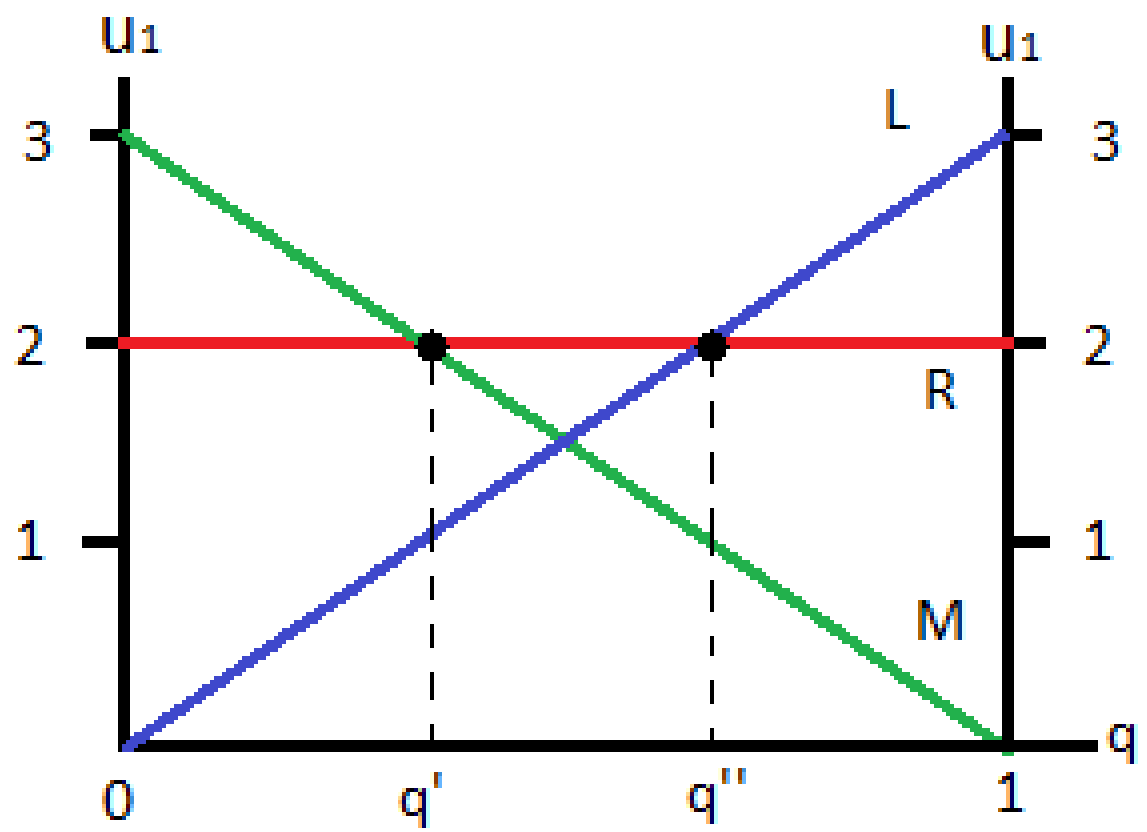
\includegraphics[width=1.1\columnwidth]{figures/Gibbons_4_2_E[u]}
      \textbf{If compatible, write up the mixed-strategy PBE.}
      \vfill\null
    \end{multicols}
\end{frame}
\begin{frame}{PS10, Ex. 6 (ii): Extensive form game (mixed-strategy PBE)}
    (ii) What is the mixed-strategy PBE? \vspace{-10pt}
    \begin{multicols}{2}
      \begin{table}
        \begin{tabular}{l|c|c|}
          \multicolumn{1}{c}{} & \multicolumn{1}{c}{L' [q]} & \multicolumn{1}{c}{R' [1-q]} \\\cline{2-3}
          L [p]   & \textcolor{red}{3}, 0 & 0, \color{blue}1 \\\cline{2-3}
          M [1-p] & 0, \color{blue}1 & \textcolor{red}{3}, 0 \\\cline{2-3}
          R       & 2, \color{blue}2 & 2, \color{blue}2 \\\cline{2-3}
        \end{tabular}
      \end{table} \vspace{-6pt}
      P1's expected utility of $L$, $M$, and $R$: \vspace{-8pt}
      \begin{align*}
        \mathbb{E}[u_1(L)|q]&=3q+0[1-q]=3q\\
        \mathbb{E}[u_1(M)|q]&=0q+3[1-q]=3-3q\\
        \mathbb{E}[u_1(R)]&=2
      \end{align*}
      P1 is indifferent at $q'$ and $q''$: \vspace{-8pt}
      \begin{align*}
        \mathbb{E}[u_1(M)]\text{=}\mathbb{E}[u_1(R)]&\Rightarrow \text{3-3}q\text{=}2\Rightarrow q'\text{=}1/3\\
        \mathbb{E}[u_1(L)]\text{=}\mathbb{E}[u_1(R)]&\Rightarrow 3q\text{=}2\Rightarrow q''\text{=}2/3
      \end{align*} \vspace{-22pt}
      \begin{align*}
        q\leq1/3&\text{:}\ BR_2(M)\text{=}L'\rightarrow\text{P1 deviates to }L\\
        q\text{$\in$}{\textstyle\left[\frac{1}{3},\frac{2}{3}\right]}&\text{:}\ \text{P1 plays }R\rightarrow\text{does P2 mix?}\\
        q\geq2/3&\text{:}\ BR_2(L)\text{=}R'\rightarrow\text{P2 deviates to }M
      \end{align*}
      P2 is indifferent if she believes that: \vspace{-8pt}
      \begin{align*}
        \mathbb{E}[u_2(L')]\text{=}\mathbb{E}[u_1(R')]&\Rightarrow \text{1-}p\text{=}p\Rightarrow p^*\text{=}1/2
      \end{align*}
      $q\in$$\left[\frac{1}{3},\frac{2}{3}\right]$: P1 plays $R$. $p=\frac{1}{2}$: P2 mixes.
      \vfill\null\columnbreak
      \begin{figure}[!h]
        \center \def\svgwidth{1.1\columnwidth}
        \import{figures/}{Gibbons_4_2_ii.pdf_tex}
      \end{figure}
      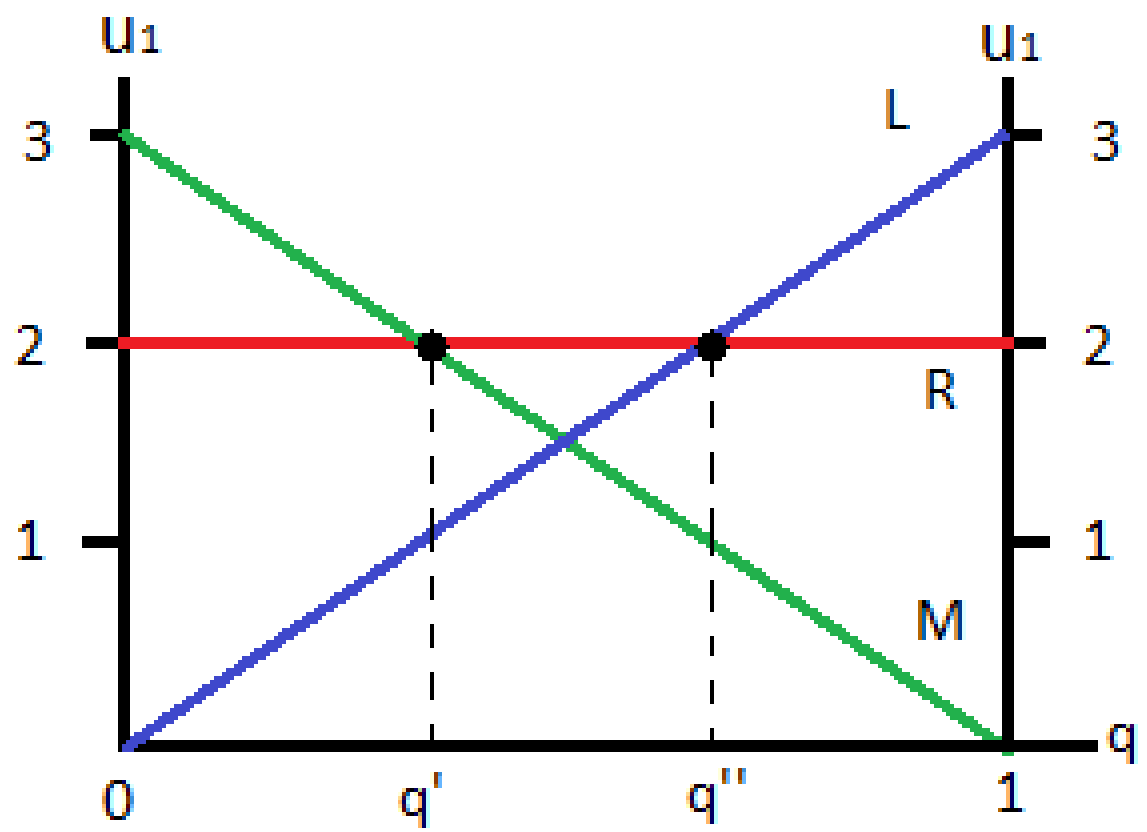
\includegraphics[width=1.1\columnwidth]{figures/Gibbons_4_2_E[u]}
      \vspace{-16pt}
      \begin{align*}
        \bm{PBE=\left\{\left(R,q\in\left[\frac{1}{3},\frac{2}{3}\right]\right),p=\frac{1}{2}\right\}}
      \end{align*}
      \vfill\null
    \end{multicols}
\end{frame}
